\chapter{Foreword}

This manual has been drafted for the V6 software release.

The information given in this manual is subject to revision without notice. EDF-R\&D disclaims any responsibility for or in relation to the contents hereof.

No copy may be made of this document, either mechanically or electronically, without the prior written consent of EDF-R\&D.

The TELEMAC-2D, TELEMAC-3D, \artemis{}, POSTEL-3D, \stbtel{}, SISYPHE, TOMAWAC, ESTEL-2D, ESTEL-3D, SPARTACUS-2D, SINUSX, EDAMOX,MATISSE and RUBENS programs are the property of EDF-R\&D

The SIMAIL program is the property of SIMULOG.

The SUPERTAB program is the property of SDRC.

The TRIGRID program is the property of the Institute of Ocean Sciences, Canada.

The FASTTABS program is the property of Brigham Young University, USA.

Copyright 2009 EDF-R\&D

\chapter{Typing conventions used in this manual}


The computational items (variable names, file names, etc.) are written in \verb!courier font!.

The keywords are written in \textit{ITALIC BOLD CHARACTERS}

The literature references are given between brackets [ ].


\chapter{Introduction}

The \artemis{} code (Agitation and Refraction with TELEMAC on a MIld Slope)
solves the Elliptic mild slope equation \cite{berkhoff1976} using finite
element techniques inside the TELEMAC modelling system structure. This equation
is obtained from the Navier-Stokes equations according a set of hypothesis (low
value of wave steepness, low value of bottom slope). The main results at each
node of the computational mesh are the height, the phase and the direction of
the wave. The main application of \artemis{} concerns the wave agitation in
harbours or small bays. ARTEMIS is able to take into account the following
phenomena :

\begin{itemize}
\item  Wave reflection by an obstacle,

\item  Wave diffraction behind an obstacle,

\item  Wave refraction by bottom variation,

\item  Regular wave,

\item  Monodirectional or multidirectional random wave,

\item  Bottom friction,

\item  Bathymetric breaking.

\item  Taking into account of the dissipation by breaking and/or bottom friction,

\item  Improvement of boundary conditions taking into account incidence angle on a solid boundary, and input/output angle in a liquid boundary,
\end{itemize}

However, the actual version of the software is unable to take into account the following phenomena:

\begin{itemize}
\item  Wave refraction by current,

\item  Dry area inside the domain (tidal flats).
\end{itemize}

The application domains of the software are various. In particular, it offers
the possibility to study wave agitation in harbour or bay, to appreciate the
impact of harbour equipment (pier, dike), to evaluate the wave agitation behind
a breach, the wave decay behind an island or flat, seiching in a channel, etc.

\artemis{} was developed by the National Hydraulics and Environnement
Laboratory (Laboratoire National d'Hydraulique et d'Environnement - LNHE) of
the Research and Studies Directorate of the French Electricity Board
(EDF-R\&D). The program complies with EDF-DER's Quality Assurance procedures
for scientific and technical programs \cite{QualityGroup1993}. This sets out rules
for developing and checking product quality at all stages. In particular, a
program covered by Quality Assurance procedures is accompanied by a Validation
File that describes a set of test cases (see reference \cite{ArtVal1997}).
This document can be used to determine the performance and limitations of the
software and define its field of application. The test cases are also used for
developing the software and are checked each time new versions are produced.
Description sheets for each test case have been updated for the version 6.2 of
the code.


\section{Situation of \artemis{} within the TELEMAC modelling system}

The \artemis{} software is part of a complete set of computational software and their associated pre- and post-processors, the TELEMAC system. This offers all the modules required for constructing a model and using it to simulate 2D and 3D hydrodynamic phenomena (wave and current), water quality and sedimentology.

The TELEMAC system comprises the following modules:

\begin{itemize}
\item  The MATISSE software designed, using the bathymetric and/or topographic
  data, to generate a mesh consisting of triangular elements,

\item  The \stbtel{} software designed to retrieve the file from a mesh
  generator, possibly interpolate a bathymetry, and generate a geometry file in
    the SELAFIN format that can be read by the simulation modules as well as
    the RUBENS software. \stbtel{} also conducts a number of mesh coherence
    checks,

\item  The TELEMAC-2D software designed to perform the hydrodynamic simulation
  in two horizontal space dimensions. In addition, TELEMAC-2D can simulate the
    transport of dissolved tracers,

\item  The TELEMAC-3D software itself, designed to carry out the hydrodynamic
  simulations of flows in three space dimensions. Besides, TELEMAC-3D can
    simulate the transport of tracers. The SEDI-3D library contains of the
    relevant subroutines for the simulation of non-cohesive sediment transport.
    The implementation of the TELEMAC-3D software is the subject matter of this
    document,

\item  The SISYPHE software designed to carry out the simulation the transport
  of sediment through bed load traction and suspension.

\item  The \artemis{} software designed to simulate the changes in the features
  of wave agitation either in a coastal water body or a harbour,

\item  The TOMAWAC software designed to simulate, through a spectral method,
  the sea state in permanent or transitory conditions,

\item  The ESTEL-2D software designed to simulate the underground flows in two
  vertical space dimensions,

\item  The ESTEL-3D software designed to simulate the underground flows in three dimensions,

\item  The POSTEL-3D software designed to prepare the 2D cross sections in the
  3D result file, for a processing by the RUBENS graphics software,

\item  The RUBENS software designed to graphically process the results of the
  various simulation modes,

\item  The SPARTACUS-2D software designed to simulate the two-dimensional
  laminar and turbulent flows through the SPH method.
\end{itemize}

As a complement to the TELEMAC chain, the FUDAA-PREPRO software (as developed
from the FUDAA platform by the CETMEF's, Informatics and Modelling Research
Department) covers all the preprocessing tasks involved by the achievement of a
digital hydraulic study.


\section{User programming}

When he uses a simulation module from the TELEMAC SYSTEM, the user may have to
program specific functions which are not provided in the code's standard
release. In particular, that is made through a number of so-called «~user~»
subroutines the sources of which are supplied within the distribution.

The procedure to be carried out in that case comprises the steps of:

\begin{itemize}
\item  Recovering the standard version of the user subroutine(s) as supplied in
  the distribution and copying it into the current directory.

\item  Amending the subroutine(s) according to the model to be constructed.

\item  Concatenating the whole set of subroutines into a single Fortran file
  which will be compiled during the \artemis{} launching process.
\end{itemize}

During that programming stage, the user can gain access to the various
variables of the software through the Fortran 90 structures.

All the data structures are gathered within Fortran files, which are known as
modules. For ARTEMIS, the file name is
\verb!DECLARATION_ARTEMIS!. To gain access to the ARTEMIS data,
just insert the command \verb!USE DECLARATIONS_ARTEMIS! into
the beginning of the subroutine. Adding the command \verb!USE BIEF! may also
be necessary in order to reach the structure in the BIEF library.

\chapter{Theoretical Aspects}

This report is the theoretical note of the scientific software \artemis{},
version 3.0. ARTEMIS deals with the modelling of wave propagation towards the
coast and wave agitation in harbours. This software is integrated in the
TELEMAC system, and is developed following the Quality Assurance procedures in
effect in the Research Division of Electricit\'{e} de France.

After a few words about the statistical and spectral approaches of the wave
description, we present the theoretical model of monochromatic waves as used by
\artemis{}, which is based on the Berkhoff's or mild slope equation verified by
the velocity potential. Then, we describe how non-linear dissipative processes
have been included in the initial linear model. The various formulations
implemented in the software to quantify the wave energy dissipation through
surf-breaking and bottom friction are explained. The treatment of liquid and
solid boundaries is realized through Neumann conditions, and enables to model
incident waves (radiation condition), free wave-output, full or partial
reflectionsreflection. A specific methodology, presented in the report, has
been developed in \artemis{} to take into account directional spreading and
frequency distribution of the wave energy (random waves). Finally, we describe
the numerical algorithm implemented to solve the mathematical model, as
expressed through the finite element formulation, using functions developed in
the BIEF library of the TELEMAC system.


\section{Main symbols and units}



\begin{tabular}{|p{0.8in}|p{0.5in}|p{3.1in}|} \hline
  $\Phi$ & m${}^{2}$s${}^{-1}$ & velocity potential \\ \hline
  $\phi$ & m${}^{2}$s${}^{-1}$ & reduced velocity potential \\ \hline
  A & m${}^{2}$s${}^{-1}$ & amplitude of reduced potential: $\phi=A e^{i\beta}$ \\ \hline
  $\beta$ & rad & phase of reduced potential: $\phi=A e^{i\beta}$ \\ \hline
  H & m & wave height \\ \hline
  H${}_{1/3}$ & m & significant wave height (statistical approach) \\ \hline
  H${}_{rms}$ & m & RMS wave height (statistical approach) \\ \hline
  H${}_{m0}$ & m & significant wave height (spectral approach) \\ \hline
  H${}_{e}$ & m & wave energy height (spectral approach) \\ \hline
  H${}_{max}$ & m & maximum wave height \\ \hline
  H${}_{m}$ & m & critical wave height at breaking point \\ \hline
  T & s & wave period \\ \hline
  T${}_{H1/3}$ & s & significant wave period \\ \hline
  T${}_{p}$ & s & wave peak period \\ \hline
  Q${}_{b}$ & - & breaking rate \\ \hline
  f${}_{w}$ & - & friction coefficient\newline  \\ \hline
  E(f,$\theta$) & kg s${}^{-1}$ & wave energy spectrum \\ \hline
  S(f,$\theta$) & m${}^{2}$ Hz${}^{-1}$ & wave variance spectrum \\ \hline
  $\omega$ & rad s${}^{-1}$ & wave pulsation \\ \hline
  f & Hz & wave frequency \\ \hline
  f${}_{p}$ & Hz & peak frequency (in random waves) \\ \hline
  k & m${}^{-1}$ & wave number \\ \hline
  h & m & water depth \\ \hline
  m & - & bottom slope \\ \hline
  L & m & wave length \\ \hline
  C & m s${}^{-1}$ & phase velocity \\ \hline
  C${}_{g}$ & m s${}^{-1}$ & group velocity \\ \hline
  g & m s${}^{-2}$ & gravity acceleration (g = 9.81 m/s${}^{2}$) \\ \hline
  E & kg s${}^{-2}$ & wave energy per unit area \\ \hline
  $\rho$ & kg m${}^{-3}$ & seawater density \\ \hline
  AIPCN &  & \textbf{A}ssociation \textbf{I}nternationale \textbf{P}ermanente des \textbf{C}ongr\`{e}s de \textbf{N}avigation \\ \hline
  AIRH &  & \textbf{I}nternationale Association of \textbf{H}ydraulics \textbf{R}esearch  \\ \hline
  BIEF &  & \textbf{BI}blioth\`{e}que \textbf{E}l\'{e}ments \textbf{F}inis (syst\`{e}me TELEMAC) \\ \hline
\end{tabular}


\section{Generals about waves}\label{waves}


\subsection{Definitions}

Waves deserve their name! Defining a "wave" does call for special care when its
specific physical variables are to be determined. A wave is defined by the
deformation of the free surface between two successive occurrences either of a
zero up-crossing or a zero down-crossing including a crest and a trough.
Depending on which one of the above conventions is adopted, the distribution of
wave heights, as defined by the differences between the elevations of the wave
crests and troughs, may be different. The period of a wave can be defined using
the symbol T.

The characteristics of the sea state (height, period\ldots) can be known from
the free surface deformation signal $\zeta$(x,y,t) as a function of horizontal
position (x,y) and time t, following two kinds of approaches, namely
statistical and spectral approaches.


\subsection{Statistical approach}\label{stat_appr}

Once symbols are chosen for defining the wave height and period, all the
recorded heights H${}_{i}$ and periods of N waves can be computed from signal
$\zeta$(x,y,t). The following parameters are then defined:


\begin{tabular}{p{0.8in}p{0.1in}p{3.5in}}
  $\overline{H}$ & : & wave height average as defined by (rarely used variable):\newline
                       $$\overline{H} = \frac{1}{N}\sum_{i=1}^{N}H_{i}$$\\
H${}_{1/n}$ & : & height average in the upper (1/n)th percentile of the wave height population \\
H${}_{1/3}$ & : & the significant height is particularly defined for n = 3 \\
H${}_{rms}$ & : & root mean square value of wave heights Hi as defined by\newline
                       $$\overline{H} = \sqrt{\frac{1}{N}\sum_{i=1}^{N}H_{i}^{2}}$$\\
H${}_{max}$ & :  & maximum recorded heigh \\
T${}_{H1/3}$ & : & average of periods T${}_{i\ }$in the upper third of the wave height population\newline  \\
T${}_{1/3}$ & : & average of periods T${}_{i}$ in the upper third of the wave period population \\
  $\bar{T}$ & : & average of all the wave periods T${}_{i}$ \\
\end{tabular}

It was found in deep water that the likeliness of a wave height
H$\mathrm{{}^\circ}$ exceeding a height H was properly approximated by such a
rule as:
\begin{equation}
  Prob(H^{\circ} \ge H) = \frac{2H}{b^{2}}e^{-\left(\frac{H}{b}\right)^{2}}
\end{equation}

The related probability density is given by the following relation:

\begin{equation}
  p(H) = e^{-\left(\frac{H}{b}\right)^{2}}
\end{equation}

It defines a so-called \textit{Rayleigh's} statistical distribution of waves.
Parameter b characterizes the population. It can be related, for example, to
the root mean square value of wave height H${}_{rms}$. This is because:

\begin{equation}
  H_{rms}^{2} = \int_{0}^{\infty}H^{2}p(H)dH
\end{equation}

That integral can easily be computed: its value is b${}^{2}$. The Rayleigh's
law is then finally written as follows:

\begin{equation}
  p(H) = \frac{2H}{H_{rms}^{2}}e^{-\left(\frac{H}{H_{rms}}\right)^{2}}
\end{equation}

The following relations are given by that wave height distribution law:

$H_{1/10} = 1.27 H_{1/3}$

$H_{1/3} = 1.60 \overline{H} = 1.416 H_{rms}$

\underbar{Note: }

These results are obtained by computing the H${}_{1/n}$ heights as follows: let H*
be such that Prob~(H${}^\circ >$H*)~=~1/n. Immediately, we
have:

$$H* = \sqrt{\ln(n)}H_{rms} $$

H${}_{1/n}$ is subsequently defined by:
\[\frac{1}{n}H_{1/n}=\int^{\infty }_{H^*}{Hp\left(H\right)dH}\]
This integral is expressed as a function of H${}_{rms}$ and leads to the above
mentioned relations.

That distribution can be highly modified in shallow water under the influence
of dissipation processes (primarily breaking). A truncated model of probability
density incorporating the concept of maximum boundary height can be adopted
(cf.~\ref{steady_rand_wave} below).

Other sea state parameters can also be set either through the statistical
analysis or from each individual wave. For further information, please refer to
\cite{SeaState}.


\subsection{Spectral Approach}

The initial step is the signal $\zeta$(x,y,t) of free surface deformation in
time over the horizontal domain being investigated. After submitting the signal
$\zeta$(x,y,t) to a generalized Fourier transform combining time and space
dependence of the free surface elevation, we can write, after Massel
\cite{Massel1996}:
%TODO: 2pipi (extra pi ?)
\begin{equation}
  \zeta(x,y,t) = \zeta_{0}(x,y) + \lim_{F\rightarrow\infty}\frac{1}{F}\int_{f=-F}^{+F}\int_{\theta=0}^{2\pi}
         \tilde{A}_{x,y}(f,\theta)
         e^{i\tilde{\psi}_{x,y}(f,\theta)}
         e^{i[2\pi\pi{f}-k(x \cos \theta - y \sin \theta )]}d{f}d{\theta}
\end{equation}

wherein:

 k is a function of f through a so-called "dispersion" relation that will be identified hereinafter

 $\theta$ denotes a propagation direction with a positive counterclockwise orientation with respect to an axis Ox

 $\tilde{A}_{x,y}(f,\theta)$ et $\tilde{\psi}_{x,y}(f,\theta)$ are obtained
 through a generalized Fourier transform applied to the three-dimension case
 \cite{Hamm1995}, ,which is actually reduced to two dimensions because of the
 dispersion relation between two dimensions. In addition,
 $\tilde{A}_{x,y}(-f,\theta)$ is the conjugate complex of
 $\tilde{A}_{x,y}(f,\theta)$.
 $\tilde{A}$ is expressed in meters.

 $\zeta_{0}(x,y)$ is the average level of the free surface, with an assumed zero value all over the domain being investigated.

The directional spectrum E(f,$\theta$) of wave energy at every point
(x,y) in the domain is related to $\tilde{A}_{x,y}(f,\theta)$ by the
following formal relation :

\begin{equation}
  E(f, \theta)dfd\theta = \frac{1}{2}\rho g\tilde{A}_{x,y}^{'2}(f, \theta)
\end{equation}

wherein  '${}_{x,y}$(f,$\theta$) = 2 ${}_{x,y}$(f,$\theta$)

The directional spectrum S(f,$\theta$) of wave action, as expressed in m${}^{2}$.Hz${}^{-1}$, is usually defined by

\begin{equation}
S(f,\theta)=E(f,\theta)/(\rho g)
\end{equation}


The following spectral wave parameters can be set from S(f,$\theta$) :

\begin{tabular}{p{0.8in}p{0.1in}p{3.5in}}
  m${}_{n}$ & : & n-order moment of directional spectrum as defined by :\newline
                  $$ m_{n} = \int_{f=0}^{+\infty}\int_{\theta=0}^{2\pi}f^{n}S(f,\theta)dfd\theta$$\\
  m${}_{0}$ & : & especially for n = 0, the variance m0 of the free surface difference of level is defined \\
  H${}_{m0}$ & : & significant spectral height, as defined by :\newline
                   $$ H_{m0} = 4\sqrt{m_{0}}$$\\
  H${}_{e}$ & : & Spectral energy height as defined by the relation :\newline
                  $$ m_{0} = \frac{1}{8}H_{e}^{2}$$
                  Thus, H${}_{e}$ is related to H${}_{m0}$ by : $$ H_{e} = \frac{H_{m0}}{\sqrt{2}}$$  \\
  T${}_{p}$ & : & peak period as determined by the maximum value of spectrum S(f,$\theta$) \\
  $\theta_{m}$ & : & mean wave direction, as defined by the expression :\newline
                   \[\theta_{m} =\frac{\int_{0}^{2\pi}\int_{f=0}^{+\infty} \theta S(f,\theta ) df d\theta}
                                 {\int_{0}^{2\pi}\int_{f=0}^{+\infty} S(f,\theta ) df d\theta} \] \\
  T${}_{0,1}$ & : & First mean spectral wave periods defined by :\newline
                   \[T_{01} =\frac{m_{0} }{m_{1} } = \frac{\int_{0}^{2\pi}\int_{f=0}^{+\infty} S(f,\theta ) df d\theta}
                                                         {\int_{0}^{2\pi}\int_{f=0}^{+\infty} f S(f,\theta ) df d\theta} \] \\
  T${}_{0,2}$ & : & Second mean spectral wave periods defined by:\newline
                   \[T_{02} =\sqrt{\frac{m_{0} }{m_{2}}} = \sqrt{\frac{\int_{0}^{2\pi}\int_{f=0}^{+\infty} S(f,\theta ) df d\theta}
                                                                      {\int_{0}^{2\pi}\int_{f=0}^{+\infty} f^{2}  S(f,\theta ) df d\theta}} \] \\
  T${}_{M}$ & : & Third mean spectral wave TM defined by:\newline
                  \[T_{M} =\frac{\int_{0}^{2\pi}\int_{f=0}^{+\infty} (1/f) S(f,\theta) df d\theta}
                                {\int_{0}^{2\pi}\int_{f=0}^{+\infty} S(f,\theta) df d\theta} \] \\
  $\bar{k}$ & : & Mean wave number, computed from the dispersion relationship using the mean pulsation $\bar{\omega}=2\pi /T_{01} $ \\
  $\bar{C}$ & : & Mean phase velocity $\bar{C}=\bar{\omega }/\bar{k}$ \\
  $\bar{C}_{g}$ & : & Mean group velocity $\bar{C}_{g} =d\bar{\omega }/d\bar{k}$ \\
\end{tabular}

As in the statistical analysis, other parameters can be computed from the
energy spectrum (see in \cite{SeaState}). If the height distribution
complies with a Rayleigh's law, then the statistical approach and the spectral
approach may correspond to each other:

$$ H_{m0} = H_{1/3} $$
$$ H_{e} = H_{rms} $$

These two approaches are not necessarily equivalent to each other in shallow
waters where the dissipation processes (mainly surf-breaking) and the
non-linear transfers between frequencies affect the distribution of wave
heights (see in \cite{Hamm1995}).


\section{Theoretical modelling}


\subsection{Concept's background. Basic assumptions}

%TODO: Missing ref to navier sto
All the wave propagation theories rely on the Newtonian fluid dynamics model as
described by the Navier-Stokes equations [7]. These general equations can more
or less be simplified according to the extent of complexity as kept by the
modelling hypothesis. We will consider how to set the Berkhoff's model
\cite{berkhoff1976} or in other word the "mid slope equation", describing the
monochromatic wave \textbf{refraction} and \textbf{diffraction} both by slowly
spatially-changing bottoms and by obstacles. Such processes as partial or total
reflection, wave inflow or outflow, are governed by boundary conditions to be
specified hereinafter.

The fluid movement is located in an Oxyz Cartesian co-ordinate system whose
axis z coincides with the ascending vertical. The origin of axis Oz is taken at
the free surface at rest. The free surface elevation and the bottom depth are
denoted $\zeta\alpha{v}\delta-h$, respectively (h being the positive or negative water
depthwater depth at rest). H is the wave height, L is its wavelength
(fig~\ref{fig:notations})

\begin{figure}[H]%
\begin{center}
%
  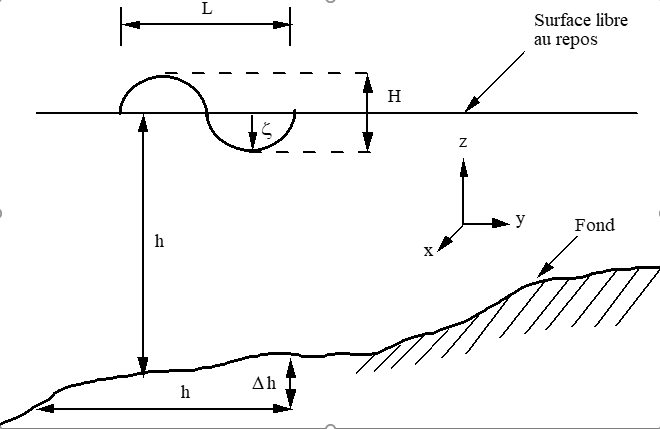
\includegraphics[width=\textwidth]{./graphics/notations}
%
\end{center}
\caption{Illustration of used notationsMixing lengths versus depth.}\label{fig:notations}
\end{figure}

The general modelling assumptions are as follows:

\begin{itemize}
\item  the fluid (seawater) is assumed to be \textit{nonviscous}

\item  the flow is assumed to be \textit{irrotational}. Thus, one can introduce
  such a potential $\Phi$ as $\nabla\Phi = \overrightarrow{u}$, wherein  $\overrightarrow{u}$ is the
    fluid particle velocity vector

\item  the fluid is assumed to be \textit{uncompressible}

\item  the bottoms do not change in time
\end{itemize}


\subsection{Development of Berkhoff's equation}


\paragraph{Forming the equations}

Once the above assumptions and definitions are available, the momentum
conservation and continuity equations can be simplified as follows:
\begin{equation}
  \nabla^{2}\Phi = 0
  \label{eq:mass_cons}
\end{equation}
\begin{equation}
  \nabla \left(\frac{\partial\Phi}{\partial t}+\frac{1}{2}(\nabla\Phi)^{2}+\frac{p}{\rho}+gz\right)=0
  \label{eq:momentum}
\end{equation}

using the conventional notations, namely p for pressure, $\rho$ for water
density and g for gravity. Equation~\ref{eq:mass_cons} expresses the
conservation of mass and Equation~\ref{eq:momentum} expresses the conservation
of momentum (as written in the form of the Bernoulli's equation). Pressure p is
not hydrostatic due to the wave action.

These two equations are associated to the boundary conditions both at the free
surface (z~=~$\zeta$) and the bottom (z = -h); the boundary conditions are
written as follows:

\begin{equation}
  \left.\frac{\partial\Phi}{\partial z}\right|_{z=\zeta(x,y,t)} =
       \frac{\partial\zeta}{\partial t} +
       \frac{\partial\Phi}{\partial x}.\frac{\partial\zeta}{\partial x} +
       \frac{\partial\Phi}{\partial y}.\frac{\partial\zeta}{\partial y}
  \label{eq:imperviousness}
\end{equation}
\begin{equation}
  \left.\frac{\partial\Phi}{\partial z}\right|_{z=-h(x,y)} =
       -\frac{\partial\Phi}{\partial x}.\frac{\partial h}{\partial x}
       -\frac{\partial\Phi}{\partial y}.\frac{\partial h}{\partial y}
  \label{eq:bottom_imp}
\end{equation}

Equation~\ref{eq:imperviousness} expresses the free surface imperviousness and
equationr~\ref{eq:bottom_imp} expresses the bottom imperviousness.

In spite of their seemingly simple form, these two sets of equations, however,
are still difficult to solve, since they include non-linear terms :


$(\nabla\Phi)^{2}$ in eq~\ref{eq:momentum}, and
$\frac{\partial\Phi}{\partial x}.\frac{\partial\zeta}{\partial x} +
 \frac{\partial\Phi}{\partial y}.\frac{\partial\zeta}{\partial y}$
 in eq~\eqref{eq:imperviousness}.

Through assumptions about the wave and bottom characteristics, these equations
will be linearized and will then be solved more easily.


\paragraph{Linearization}

That linearization is conducted under the following assumptions :

\begin{itemize}
  \item  \textit{Gentle steepness: $\epsilon_{1}=H/L << 1$}
  \item \textit{small wave height against depth: $\epsilon_{2}=H/h << 1$ }
\end{itemize}

The solution $\Phi_{0}$~=~0 and $\zeta_{0}$~=~0 (i.e.\ rest) is a
particular solution to the problem. Further solutions disturbing that
particular solution will be searched for. The following linear system is
achieved through a series development of the potential, only keeping 1-order
terms in $\epsilon_{1}$ :

\begin{equation}
  \nabla^{2}\Phi = 0
  \label{eq:3.12}
\end{equation}
\begin{equation}
  \text{en z = 0} \frac{\partial \Phi}{\partial t} + g\zeta = 0
  \label{eq:3.13}
\end{equation}
\begin{equation}
  \text{en z = 0} \frac{\partial \Phi}{\partial z} = \frac{\partial \Phi}{\partial t}
  \label{eq:3.14}
\end{equation}

\begin{equation}
  \text{en z = -h(x,y)} \frac{\partial \Phi}{\partial z} =
    - \frac{\partial\Phi}{\partial x}.\frac{\partial h}{\partial x} +
    - \frac{\partial\Phi}{\partial y}.\frac{\partial h}{\partial y}
  \label{eq:3.15}
\end{equation}

In order to derive Equation~\ref{eq:3.13}, the Bernoulli's equation at
the surface (Equation~\ref{eq:momentum}) was written. Pressure is then the
air pressure, i.e.\ a constant pressure. Thus, it disappears from the equation,
since its gradient is null

We have at the surface (i.e.\ in z = 0, since the free surface distortions are
ignored to 0-order in the series development in $\epsilon_{1}$):

\[ \nabla(\frac{\partial \Phi}{\partial t}+g\zeta) = 0\]

Or also:

\[ \frac{\partial \Phi}{\partial t}+g\zeta = \lambda(t)\]


wherein $\lambda$ function is only time-dependent. That function can be
introduced into the time derivative of the potential. This is because the
physical quantity herein is velocity, which remains unchanged when a term that
is only time-dependent is added to the potential.

By deleting $\zeta$ between equations~\ref{eq:3.13} and~\ref{eq:3.14}, one
finally comes to:

\begin{equation}
  \nabla^{2}\Phi = 0
  \label{eq:3.16}
\end{equation}
\begin{equation}
  \text{en z = 0} \frac{\partial^{2} \Phi}{\partial^{2} z} + g\frac{\partial \Phi}{\partial z} = 0
  \label{eq:3.17}
\end{equation}
\begin{equation}
  \text{en z = -h(x,y)} \frac{\partial \Phi}{\partial z} =
    - \frac{\partial\Phi}{\partial x}.\frac{\partial h}{\partial x} +
    - \frac{\partial\Phi}{\partial y}.\frac{\partial h}{\partial y}
  \label{eq:3.18}
\end{equation}

The linear theory is derived from equations~\eqref{eq:3.16},~\eqref{eq:3.17}
and~\eqref{eq:3.18}, by separating t and z variables as well as x and y
variables.

Considering the problem to be solved, the vertical component z probably does
not play the same part as components x and y. Furthermore, since the equations
are linear, every potential can be broken down into a time Fourier series. One
may only study the complex potential functions in $e^{-i\omega{t}}$. $\Phi$
will then be searched for as follows:
\begin{equation}
  \Phi(x,y,z,t) = f (z,h).\phi(x,y,z).e^{-i\omega{t}}
\end{equation}

A complex notation is used for computing the unknown functions. The return to physical quantities takes place by taking the real part of the complex variables. It is noteworthy that if h is not constant, f, like $\phi$, depends on z, as well as of x and y through h.


\paragraph{Solution in case of a horizontal flat bottom}

In case of an infinite, horizontal flat bottom, then f only depends on z and
$\phi$ only depends on x or y (e.g.\ x). The solution to the problem is in the
following form:

\begin{equation}
  \Phi(x,y,z,t) = -i \frac{gH}{2\omega}.\frac{ch(k(z+h))}{ch(kh)}.e^{i(k.x-\omega t)}
  \label{eq:3.20}
\end{equation}

That potential describes the propagation of a monochromatic monodirectional
wave (first-order Stokes' wave). Quantities k, h, g and $\omega$ are related to
each other by the dispersion function (i.e.\ Airy's relation):

\begin{equation}
  \frac{\omega^{2}}{gk} = th(kh)
  \label{eq:3.21}
\end{equation}

Note: so-called evanescent modes, which can play a significant part near the
obstacles, are solutions in the form
$cos[p_{n}(z+h)](A_{n}e^{p_{n}x}+B_{n}e^{-p_{n}x})$ , which can be added to
that general-purpose solution. Parameters p${}_{n}$ are then solutions to the
following transcendent equation:

\begin{equation}
  -\omega^{2} = gp_{n}\tan(p_{n}h)
\end{equation}

\paragraph{Solution in case of a low variation bottom (Mild-slope equation)}\label{low_var_bot}

In order to solve the problem resulting from linearized
equations~\eqref{eq:3.16} to~\eqref{eq:3.18} in case of a spatially-varying
bottom, a further assumption will be made:

\[ \epsilon_{3} = \frac{\Delta h/h}{h/L} << 1 \]

Wherein $\Delta$h denotes the bottom depth variation over a horizontal distance
such as h (refer to the diagram below).

It can be assumed from that inequality that the bottom slope
$\tan\alpha_{1}$ remains lower by an order of magnitude than the slope as
defined by the h/L~=~tan~$\alpha_{2}$ ratio (refer to the diagram below):


\begin{figure}[H]%
\begin{center}
%
  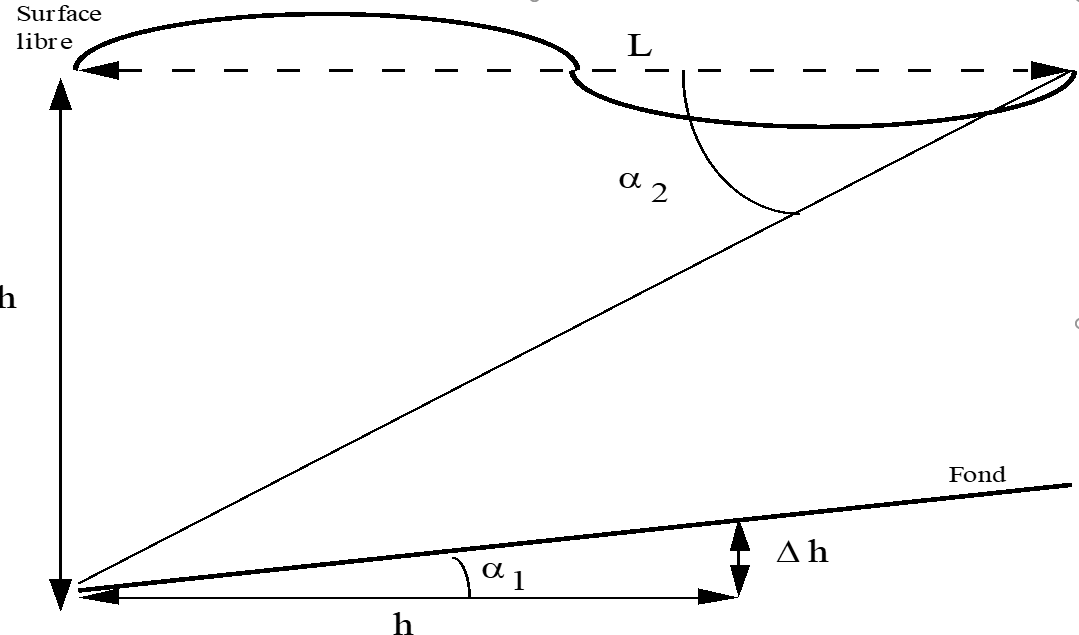
\includegraphics[width=\textwidth]{./graphics/lowvariation_bottom}
%
\caption{Illustration of a low variation bottom}\label{fig:notations}
\end{center}
\end{figure}

Through that additional assumption, Berkhoff~\cite{berkhoff1976}, develops the
solution of equations by looking for such a solution as:

\begin{equation}
  \Phi(x,y,z,t) = \frac{ch(k(z+h)}{ch(kh)}\phi(x,y)e^{-i\omega t}
  \label{eq:3.23}
\end{equation}

This is a product of three terms. The first one is related to function f
((refer to Equation \eqref{eq:3.20}. It is the same as the solution
achieved for a horizontal flat bottom, which is suitable in that case since
bottom changes slowly. The second term $\phi$ is looked for as independent from
z to the first order in $\epsilon_{3}$ and is called a reduced potential.
The third term means that time-periodic solutions are being searched for.

On completion of computations, Berkhoff obtains a general-purpose equation as
confirmed by the reduced potential $\phi$:

\begin{equation}
  \nabla(CC_{g}\nabla\phi)+CC_{g}k^{2}\phi = 0
  \label{eq:3.24}
\end{equation}

wherein:

\begin{itemize}
\item  C and C${}_{g}$ denote the phase and group velocities, respectively

\item  k denotes the wave number: k=2$\pi$/L

\item  $\nabla$ and $\nabla$ denote the gradient and divergence operators, respectively, as
  restricted to the horizontal co-ordinates
\end{itemize}

The unknown $\phi$ is an a priori complex number. Velocities are expressed from
the theory as achieved for the case of a horizontal bottom:

\begin{equation}
  C = \frac{\omega}{k}
  \label{eq:3.25}
\end{equation}
\begin{equation}
  C_{g} = \frac{1}{2}\left[1+\frac{2kh}{sh(2kh)}\right]C
  \label{eq:3.26}
\end{equation}

The mild-slope equation is a two-dimension model making to possible to take
into account the effects of refraction by bathymetry which is assumed to
exhibit slow variations in space, as well as the effects of diffraction by both
above-water and under-water obstacles. The total or partial reflection
processes are taken into account in the imposed boundary conditions. Energy
should also be supplied to the flow domain, since there is no source term in
Equation~\eqref{eq:3.24}. The boundary conditions make it possible to
satisfy that requirement, as well as to freely release the wave energy. That
model represents the propagation of steady waves, what means that the whole
wave energy is contained in only one frequency. The way that mild-slope model
of monochromatic wave can be used for describing a random wave behaviour will
be discussed in~\ref{random_mono}.


\paragraph{Solution in case of rapidly varying topography}

Since version 6.1, ARTEMIS can take into account effects of a rapidly varying
topography in the mild-slope equation.

ARTEMIS use the work presented in~\cite{Michel1999}. Second order terms from
gradient and curvature are integrated in the mild-slope equation. The
refraction-diffraction equation becomes:
\[\nabla \left(CC_{g} \cdot \nabla \phi \right)+CC_{g} \left(k^{2} \cdot \left(1+f\right)+ik\mu \right)\phi =0\]
with $f=E_{1} (kh)\cdot \left(\nabla h\right)^{2} +\frac{E_{2} (kh)}{k_{0} } \cdot \Delta h$

and k${}_{0}$ is the wave number for infinite depth.

%TODO Missing link
The first term represents gradient effects and the second deals with curvature
of the bottom. It is possible for the user to only take into account gradient
effects. One can also choose to take into account only curvature effects
(see~\ref{missing_label}).

Several expressions have been proposed for E1 and E2 functions, by different
authors: Massel~\cite{Massel1993} Chamberlain and Porter~\cite{Porter1995},
Chandrasekera and Cheung~\cite{Chandrasekera1997}, Suh Lee and
Park~\cite{Suh1997}. In ARTEMIS, Chamberlain and Porter expressions have been
considered, as recommended by~\cite{Michel1999}.
\[E_{1} \left(kh\right)=\frac{\left\{x^{4} +4x^{3} \sinh (x)-9\sinh (x)\sinh (2x)+3x\left(x+2\sinh (x)\right)\cdot \left(\cosh ^{2} (x)-2\cosh (x)+3\right)\right\}}{6n\left(x+\sinh (x)\right)^{3} } \]
\[E_{2} \left(kh\right)=\frac{\left\{\sinh (x)-x\cdot \cosh (x)\right\}}{4n\cdot \cosh ^{2} (x/2)\cdot \left(x+\sinh (x)\right)} \]
$n=\frac{1}{2} \left(1+\frac{x}{\sinh (x)} \right)$

\[x=2kh\]

\paragraph{Return to physical quantities}

Once the complex reduced potential $\phi$(x,y)~=~$\phi_{r}$ +
i.$\phi_{i}$ is computed from Equation \eqref{GrindEQ__3_24_}, it becomes
possible to return to total potential $\Phi$(x,y,z,t) and to derive all the
wave characteristics from it :

Wave height

Wave height is proportional to the $\phi$ module and is given by:

\begin{equation}
  H = \frac{2\omega}{g}\left|\phi\right|
  \label{eq:3.27}
\end{equation}

\textit{Wave phase}

Wave phase $\psi$, define in $]-\infty ; \infty]$ interval , is the argument in $\phi$.It
is obtained first by computing the variable $\psi*$:

\[ \Psi^{*} \arctan\left(\frac{\phi_{i}}{\phi_{r}}\right)\]


\[ \left. \begin{matrix}\text{if } \phi_{i} < 0 \\ \text{if } \phi_{r} < 0 \end{matrix}\right\} \Psi = \psi^{*} - \pi\]
\[ \left. \begin{matrix}\text{if } \phi_{i} > 0 \\ \text{if } \phi_{r} < 0 \end{matrix}\right\} \Psi = \psi^{*} + \pi\]
\[ \text{ otherwise } \Psi = \Psi^{*} \]


\textit{Free surface elevation}

Free surface elevation is expressed by:

\begin{equation}
  \begin{aligned}
    \zeta & = -\frac{1}{g}Re\left(\partial(\frac{\phi e^{-i\omega t}}{\partial t}\right) \\
          & = - \frac{\omega}{g}(\phi_{i}\cos \omega t - \phi_{r}\sin \omega t)
  \end{aligned}
  \label{eq:3.28}
\end{equation}

\textit{Surface} \textit{velocity}

Surface velocity is expressed as the total gradient of the potential function, i.e.:

\[ \overrightarrow{V} = \left(\begin{matrix} u\\ v\\ w\end{matrix}\right) = Re(\nabla(\phi.f.e^{-i\omega t}))\]

then:

\begin{equation}
  u = \frac{\partial \phi_{r}}{\partial x}\cos\omega t +\frac{\partial \phi_{i}}{\partial x}\sin\omega t
  \label{eq:3.29}
\end{equation}
\begin{equation}
  v = \frac{\partial \phi_{r}}{\partial y}\cos\omega t +\frac{\partial \phi_{i}}{\partial y}\sin\omega t
  \label{eq:3.30}
\end{equation}
\begin{equation}
  w = \frac{\omega^{2}}{g}(\phi_{r}\cos\omega t+\phi_{i}\sin \omega t)
  \label{eq:3.31}
\end{equation}

\textit{Wave incidence}

The hodograph of horizontal surface velocity at each point is in the form of a
centered ellipse. Comparing with the major axis, the minor axis is negligible
in a rectilinear propagation area; the ellipse is then nearly rectilinear. On
the other hand, as soon as cross waves are observed, no main propagation
direction can be really distinguished any longer and the minor axis-to-major
axis ratio is no longer close to zero. It was decided in ARTEMIS to define the
wave incidence from the direction of the ellipse's major axis, in the direction
in which the free surface elevation is positive.

A simple transformation is made in order to achieve a reduction to:

\[ u = A\cos(\omega t - \varphi_{1})\]
\[ u = B\cos(\omega t - \varphi_{2})\]

Two different cases are then considered:

\begin{itemize}
  \item  if $|\varphi_{2} - \varphi_{1}| = 0$ or $\pi$, then polarization is
    linear : the ellipse is nothing but a direction segment whose tangent to
    axis (Ox) has a B/A value, to within the sign.

\item  otherwise, polarization is elliptical. Through a change in time origin
  made by setting the equations can be written in the form :
\[ u = A\cos(t')\]
\[ u = B\cos(t' - \varphi)\]
\end{itemize}

The direction of major axis is obtained by maximizing the square of velocity
module. After computing the derivative for determining the extrema, it can be
found that the minimum and maximum velocity module $\overrightarrow{V}(t'=t'_{0})$ s obtained for phase
t'${}_{0}$ verifying:

\[ \tan 2t'_{0} = \frac{B^{2}\sin 2\varphi}{A^{2}+B^{2}\cos 2\varphi} \]


That equation defines four possible phases t'${}_{0}$ corresponding in pairs to the major axis and the minor axis, respectively. Only one solution per axis is kept with the relation:

\[ t'_{0} = \frac{1}{2}\arctan\left(\frac{B^{2}\sin2\varphi}{A^{2}+B^{2}\cos2\varphi}\right)+n\frac{\pi}{2} \text{ with } n \in \{0,1\}\]

and the square of velocity module is computed for these values of t'${}_{0}$ to
clear up the uncertainty about n by selecting the value for which there is a
maximum velocity. Lastly, the incidence direction is selected by prescribing a
positive free surface elevation at time t corresponding to phase t'${}_{0}$.

\textit{Wave energy}

Wave energy per unit horizontal free surface is expressed by the following formula:

\begin{equation}
  E = \frac{1}{8}\rho gH^{2} = \frac{1}{2}\frac{\rho\omega^{2}|\phi|^{2}}{g}
  \label{eq:3.32}
\end{equation}

One half of it consists of potential energy, whereas the other half comprises kinetic energy.

The mild-slope model is a \textit{linear} model, since if $\phi_{0}$ is a
solution to Equation~\eqref{eq:3.24}, then A.$\phi_{0}$ is also a
solution $\forall A\in R$. This is an important feature that evidences the
limitations of that model when the bottoms have a small depth. This is because,
if the bottoms come up, the shoaling process will "swell" the wave heightwave
height to such an extent that it will become inconsistent with the variable
water depth. In order to improve the domain validity and to broaden
the range of applications of \artemis{}, we have amended the initial
mild-slope equation in order to take into account the prevailing dissipative
processes in shallow water, namely \textbf{bathymetric breaking} and
\textbf{bottom friction}.


\subsection{Amended mild-slope equation}

In order to take into account the dissipative effects resulting from
\textbf{bathymetric breaking} and \textbf{bottom friction},
Booij~\cite{Booij1981} and De~Girolamo \textit{et al.}~\cite{Girolamo1988}
suggest modifying the mild-slope Equation~\eqref{eq:3.17} by introducing
an additional complex term:

\begin{equation}
  \nabla(CC_{g}\nabla\phi)+CC_{g}(k^{2}+ik\mu)\phi = 0
  \label{eq:3.33}
\end{equation}

If the reduced potential is broken down in the form: $Ae^{i\beta}$ (A~being the potential
amplitude and $\beta$~being the potential phase), the previous equation leads,
through a distinction between real part and imaginary part, to an eikonal
equation that is verified by the phase:

\begin{equation}
  (\nabla\beta)^{2} = k^{2} + \frac{\nabla.(CC_{g}\nabla A)}{CC_{g}A}
  \label{eq:3.34}
\end{equation}

and to a balance equation between the energy flow and the dissipation, in the following form :

\begin{equation}
  div\left(A^{2}C_{g}\frac{\nabla\beta}{|\nabla\beta|}\right) = -\mu C_{g}A^{2}
  \label{eq:3.35}
\end{equation}

It is an energy flow balance equation to within the "$\rho$g/2" term.
Coefficient $\mu$ is a dissipation coefficient expressed in m${}^{-1}$. The
rate D of energy dissipation is expressed by the following relation:

\begin{equation}
  D = \frac{1}{2}\rho g A^{2} \mu C_{g}
  \label{eq:3.36}
\end{equation}

Several models are provided in Section~\ref{dissipation_coff} for computing the
dissipation coefficient $\mu$, depending on whether wave energy is dissipated
through breaking and/or bottom friction.


\section{Formulation of the dissipation coefficient}\label{dissipation_coeff}


\subsection{Surf-breaking }


\paragraph{Theoretical approaches }

Surf-breaking occurs when the velocity of a water particle at the free surface
exceeds the wave propagation velocity. That criterion may result in the
determination of a critical breaking height Hm  (Miche's criterion~\cite{Mei1983}) :

\begin{equation}
  H_{m} = \frac{0.88}{k}th\left(\frac{\gamma_{s}}{0.88}kh\right)
  \label{eq:3.37}
\end{equation}

A critical wave height $H_{m}$ is related to each water depthwater
depth h. Coefficient $\gamma_{s}$ takes the bottom slope m into account.
The following dependence can be suggested~\cite{Hamm1995} :

\begin{equation}
  \gamma_{s} = \frac{b}{1+a\frac{h}{gT^{2}}}
\textbf{with :   }
  \left\{\begin{matrix}
    a = 43.75(1-e^{-19m}) \\
    b = 1.56(1+e^{-19.5m}) \\
  \end{matrix}\right.
  \label{eq:3.38}
\end{equation}

Coefficient $\gamma_{s}$ is assumed to be constant in \artemis{}; it is given
by the user (typical value: $\gamma_{s}$~=~0.8)

Two theoretical approaches are proposed and incorporated into \artemis{} for assessing the wave-induced dissipation of energy

\begin{itemize}
\item  The former, as proposed by Dally \textit{et al.} \eqref{GrindEQ__15_}, is obtained from surf-breaking along a sloping beach and subsequent wave propagation over a flat, horizontal bottom. It consists in assuming that the divergence of wave energy flow can be assessed through :

\begin{equation}
  \frac{\partial P}{\partial x} = \frac{\partial(E.C_{g})}{\partial x} = \frac{(E.C_{g})_{s}-(E.C_{g})}{l_{s}}
  \label{eq:3.39}
\end{equation}
   (3.39)

wherein x denotes the energy propagation direction. Index "s" corresponds to a
    stable area at the end of a length l${}_{s}$ beyond the surf-breaking area.
    That length is a priori not known. The earlier authors proposed to write:

    \[ l_{s} = \frac{h}{K}\]

For a given water depth h, the more sloping is the bottom, the higher is K, and
    thus the lower is l${}_{s}$. Then the authors suggest the following
    approximations:

    $(C_{g})_{s} \approx C_{g} $

    $(H)_{s} \approx \Gamma.h$

In that case, dissipation D can be assessed:

    \begin{equation}
      D = \frac{1}{8}\rho gC_{g}FH^{2}\frac{K}{H}\left[1-\left(\frac{\gamma h}{H}\right)^{2}\right]
      \label{eq:3.40}
    \end{equation}

and, lastly, the dissipation coefficient $\mu$ is given by :

    \begin{equation}
      \mu = \frac{K}{H}\left[1-\left(\frac{\gamma h}{H}\right)^{2}\right]
      \label{eq:3.41}
    \end{equation}

Dally \textit{et al.} \eqref{Dally1984} recommend the following values for K
    and $\Gamma$ according to the bottom slope

    \begin{tabular}{|c|c|c|}
      \hline
      bottom slope & K & $\gamma$ \\ \hline
      1/80 & 0.100 & 0.350 \\ \hline
      1/65 & 0.115 & 0.355 \\ \hline
      1/30 & 0.275 & 0.475 \\ \hline
    \end{tabular}

\item  The latter approach, as proposed by Battjes \& Janssen
  \eqref{Battjes1978}, is based upon the analogy between the surf-breaking area
    and the hydraulic jump.

    \begin{minipage}[b]{0.4\textwidth}
      \begin{figure}[H]%
        \centering
        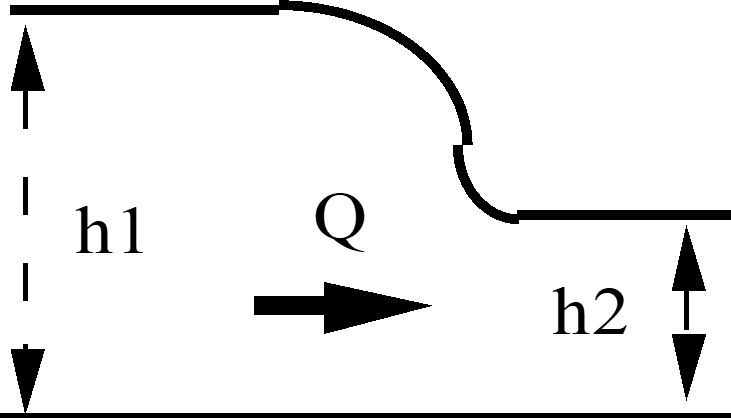
\includegraphics[width=\textwidth]{./graphics/jump}
      \end{figure}
    \end{minipage}%
    \begin{minipage}[b]{0.4\textwidth}
The head loss related to the opposite schematic jump is:
    \begin{equation}
      \Delta h = \frac{(h_{1}-h_{2})^{3}}{4h_{1}h_{2}}
      \label{eq:3.42}
    \end{equation}
The power dissipation is then:
\[ \epsilon = \rho g(\Delta h)Q  \]
Wherein $\Delta{h}=h1-h2$ \\
\end{minipage}

Q is the flow rate through the jump per unit width of channel. From the jump
conjugation relation, we have:
\begin{equation}
  Q = \sqrt{\frac{gh_{1}h_{2}(h_{1}+h_{2})}{2}}
  \label{eq:3.43}
\end{equation}

Assuming that $h_{1} \approx h_{2} \approx h$, and writing $H=h_{1}-h_{2}$, we finally have:

\begin{equation}
  \epsilon \approx \frac{1}{4}\rho g H^{3}\sqrt{\frac{g}{h}}
  \label{eq:3.44}
\end{equation}

When these results are applied to waves with a height H, a frequency f and a
length L, the power dissipation per unit area is:

\begin{equation}
  D = \frac{\epsilon}{L} \approx \frac{1}{4}\rho gf \frac{H^{3}}{h}
  \label{eq:3.45}
\end{equation}

thus:

\begin{equation}
  \mu = 2f\frac{H}{hC_{g}}
  \label{eq:3.46}
\end{equation}
\end{itemize}

Both models as described in this section are incorporated into \artemis{} software.

\paragraph{Steady wave / random wave}\label{steady_rand_wave}

When steady waves are processed using \artemis{}, either abovementioned
formulation for expressing the dissipation coefficient can be selected. That
coefficient has to be incorporated into the mild-slope equation (refer to
Equation~\eqref{eq:3.33}).

In the case of random waves, the Battjes \& Janssen's formulation alone can be
applied. Due to surf-breaking, the distribution of wave heights does no longer
follow such a Rayleigh's probability distribution as that described in
Section~\ref{stat_appr}. Battjes \& Janssen \eqref{Battjes1978} suggest that the Rayleigh's
distribution should be truncated from critical height H${}_{m}$. The
probability Q${}_{b}$ that the wave height should be equal to critical height
H${}_{m}$ is given by the following implicit relation:

    \begin{minipage}[b]{0.4\textwidth}
      \[ \frac{1-Q_{b}}{\ln Q_{s}} = \left( \frac{H_{rms}}{H_{m}}\right)\]

    \end{minipage}%
    \begin{minipage}[b]{0.4\textwidth}
      \begin{figure}[H]%
        \centering
        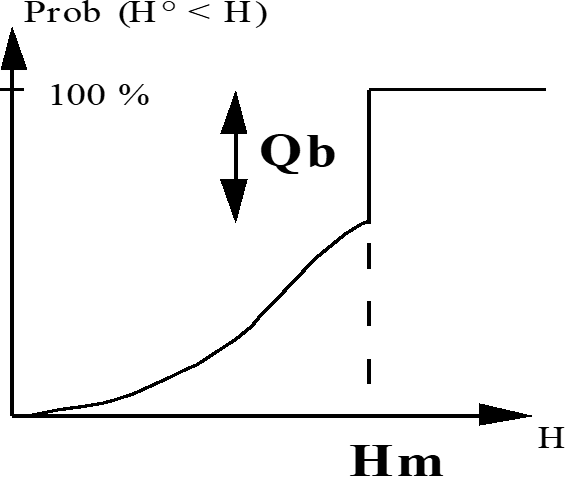
\includegraphics[width=\textwidth]{./graphics/wave_prob}
      \end{figure}
    \end{minipage}%

The rate of breaking Q${}_{b}$Q${}_{b}$ is implicitly computed in \artemis{}
through an iterative procedure. Peak frequency f${}_{p}$ is chosen as the
spectrum representative frequency. In addition, it is assumed that
H${}_{m}$H${}_{m}$~$\mathrm{\approx}$~h. Dissipation is then expressed as:

\begin{equation}
  D = \frac{\alpha}{4} Q_b f_p \rho gH_m^2
  \label{eq:3.47}
\end{equation}

and the dissipation coefficient as :

\begin{equation}
  \mu = \frac{2\alpha\alpha_pQ_b}{C_g}\left(\frac{H_m}{H_{rms}}\right)^2
  \label{eq:3.47}
\end{equation}

The value of coefficient $\alpha$ to be selected is one or so. It is set in \artemis{}.


\subsection{Bottom friction}


\paragraph{Theoretical approach}

Waves exert on the bottom a shear stress $\overrightarrow{\tau}_{b}$ that can
be expressed in accordance with the following quadratic law
(Jonsson,~\cite{Jonsson1966}):

\begin{equation}
  \overrightarrow{\tau}_{b} = \frac{1}{2}f_w\rho|\overrightarrow{U}_b|\overrightarrow{U}_b
  \label{eq:3.49}
\end{equation}

wherein f${}_{w}$ is a friction coefficient which depends on the
nature of bottoms, is the instantaneous orbital velocity just above the bottom
boundary layer. The mean energy dissipation over a wave period related to that
stress is:

\begin{equation}
  D = \frac{1}{T} \int_0^T\overrightarrow{\tau}_{b}\overrightarrow{U}_b dt
  \label{eq:3.50}
\end{equation}

\begin{itemize}
\item  For computing that integral,  Kostense et alKostense \textit{et
  al}.~\cite{Kostense1986} linearised the expression of bottom friction by
    introducing the dissipation coefficient $\mu$, the water depth h and the
    surface orbital velocity $\overrightarrow{U}_b$:
\end{itemize}

\begin{equation}
  \overrightarrow{\tau}_{b} = \rho\mu C_g h\overrightarrow{U}
  \label{eq:3.51}
\end{equation}

From these two expressions of $\overrightarrow{\tau}_{b}$, they derived a
formulation of the dissipation coefficient for friction:

\begin{equation}
  \mu = \frac{1}{2}\frac{f_w}{C_g \cos^2 (kh)}U_e
  \label{eq:3.52}
\end{equation}

wherein U${}_{e}$ is an effective velocity representing the flow and being
given by the following ration:

\begin{equation}
  U_e = \frac{\int_0^T|\overrightarrow{U}|^3}{\int_0^T|\overrightarrow{U}|^2}
  \label{eq:3.53}
\end{equation}

Accurately computing the value of U${}_{e}$ is a heavy task. We have
incorporated an approximate, quick computation of that variable into \artemis{}
(see in~\cite{Paugam}):

\begin{equation}
  U_e \approx 1.2\sqrt{\frac{1}{2}\left[
          \left(\frac{\partial \phi_r}{\partial x}\right)^2 +
          \left(\frac{\partial \phi_i}{\partial x}\right)^2 +
          \left(\frac{\partial \phi_r}{\partial y}\right)^2 +
          \left(\frac{\partial \phi_i}{\partial y}\right)^2
                                  \right]}
  \label{eq:3.54}
\end{equation}

The error made through that approximation does not exceed 15~\%.

\begin{itemize}
\item  Putnam \& Johnson~\cite{Putnam1949} simplified the computation of
  dissipation by assuming that the near-bottom orbital velocity U${}_{b}$ was
    suitably described by the results of Stokes' waves on a flat bottom (see in
    Section~\ref{low_var_bot}). An expression is easily derived for dissipation
    coefficient $\mu$ :
\end{itemize}

\begin{equation}
  \mu = \frac{2}{3\pi}\frac{f_w H \omega^3}{gC_g \sinh^3(kh)}
  \label{eq:3.55}
\end{equation}
   (3.55)

Both above formulations are incorporated into \artemis{}; the user chooses
either formulation. The friction coefficient f${}_{w}$f${}_{w}$ is still to be
determined. In the case of sandy bottoms, a number of authors proposed
assessment methods for the computation of f${}_{w}$f${}_{w}$. We have adopted
for \artemis{} the Van Rijn's approach~\cite{vanRijn1993} which consists in
determining f${}_{w}$ as a function of a Reynolds number which is computed both
from the excursion of a fluid particle over the bottom and a relative
roughness, which takes into account the grain (or skin) roughness, the shape
roughness if ripples appear, as well as from the excursion of fluid particles
over the bottom. When the bottoms are not sandy or if the user does not want to
apply the above procedure, the value of f${}_{w}$ over the computational domain
can be specified, whether a space-uniform or space-variable value is chosen.

The typical values of f${}_{w}$ are : 10${}^{-3}$ or so for a smooth concrete bottom ; 10${}^{-2}$ for a gravel bottom ; 10${}^{-1}$ for stones, rocks.

Note:

\begin{itemize}
\item  Dissipation through bottom friction is low as compared with
  breaking-induced dissipation and is exerted over long distances.
    Breaking-related dissipation is greater, but spatially localized.

\item  Both for breaking and bottom friction, coefficient $\mu$ depends on
  height H, and then on potential $\phi$ which is a priori unknown. That
    dependence cannot be implicitly solved through a matrix system. We have
    therefore incorporated a new algorithm of such a kind as the "firing
    procedure" algorithm provided for solving the potential when some
    dissipation occurs. That algorithm is discussed in Section~\ref{digi_sol}.
\end{itemize}


\section{Boundary conditions}

In order to be mathematically and physically well formulated, the problem to be
solved should take into account the prescribed conditions at the boundaries of
the domain being investigated. Physically, there can be two kinds of boundaries:

\begin{itemize}
\item  either \textit{solid boundaries} fully or partly reflecting the waves
  (breakwaters, quays, beaches\ldots);

\item  or openings facing the open sea or an inner dock (\textit{liquid
  boundaries}) through which waves flow in or out.
\end{itemize}

These kinds of boundary conditions should mathematically be expressed in the
computation unknown, i.e.\ the reduced potential $\phi$.


\subsection{Solid boundaries}

The instance when waves come against a wall and have a main direction of
propagation which makes an angle $\theta_{p}$ to the normal outside the
wall (refer to Fig~\ref{fig:reflex} below) will now be contemplated:

\begin{figure}[H]%
\begin{center}
%
  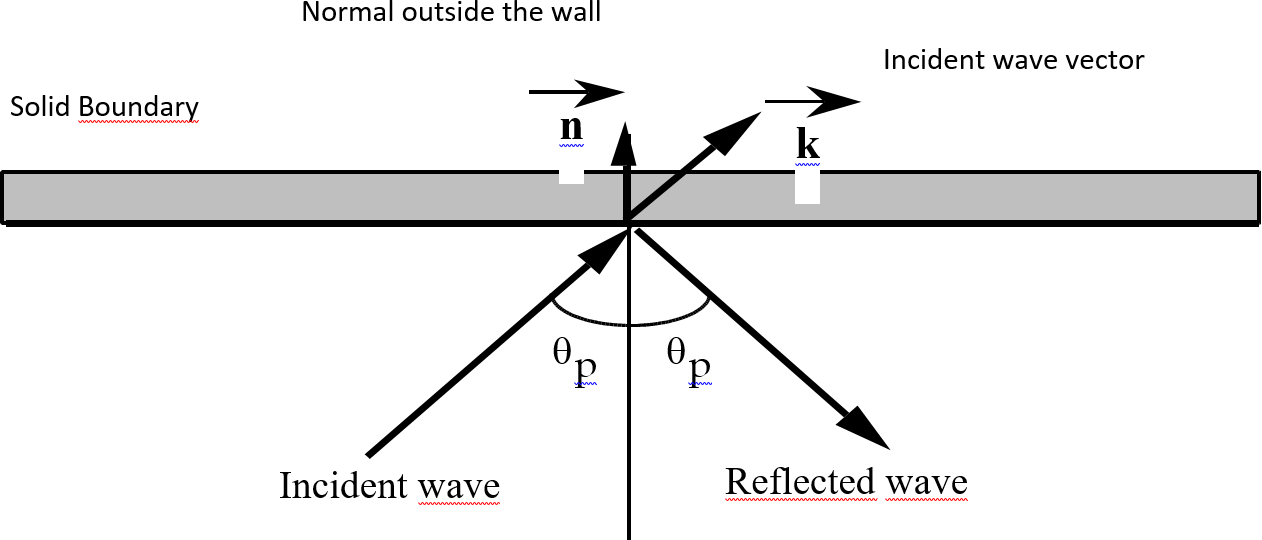
\includegraphics[width=\textwidth]{./graphics/reflex}
%
\caption{Definition of reflexion angles}\label{fig:reflex}
\end{center}
\end{figure}

In front of that wall, incident waves and reflected waves, corresponding to
potentials $\phi_{inc}$ and $\phi_{ref}$ are superposed on
each other. The reflection process is modelled through a relationship
between potentials $\phi_{inc}$ and $\phi_{ref}$. Let the
wall reflection coefficient, which is a priori complex, be called
Re${}^{i}$. Then it expresses not merely a loss of amplitude upon the
reflection from the wall (coefficient R), but also a wall-induced time lag
(coefficient $\alpha$).

At the wall, velocities and elevations of free surface incident and reflected
waves are related by:

%TODO: missing left{
\begin{equation}
  \overrightarrow{u}_{ref}.\overrightarrow{n} = -Re^{i\alpha}\overrightarrow{u}_{inc}.\overrightarrow{n}
  \label{eq:3.56}
\end{equation}
\begin{equation}
  \zeta_{ref} = Re^{i\alpha}\zeta_{inc}
  \label{eq:3.57}
\end{equation}

or also, taking as the incident wave a traveling monodirectional wave in the
form: $e^{i(\overrightarrow{k}\overrightarrow{x}-\omega t}$ :

%TODO: missing left{
\begin{equation}
  \frac{\partial \phi_{ref}}{\partial n} = -Re^{i\alpha}e^{i(\overrightarrow{k}_{ref}-\overrightarrow{k}_{inc})}
           \frac{\partial\phi_{inc}}{\partial n}(\text{car}\overrightarrow{k}_{inc}.\overrightarrow{n} = -\overrightarrow{k}_{ref}.\overrightarrow{n})
  \label{eq:3.58}
\end{equation}
\begin{equation}
  \phi_{ref} = Re^{i\alpha}e^{i(\overrightarrow{k}_{ref}-\overrightarrow{k}_{inc})}\phi_{inc}
  \label{eq:3.59}
\end{equation}

and, by replacing $\phi_{ref}$ with $\phi-\phi_{inc}$, we finally get:
\begin{equation}
  \frac{\partial \phi}{\partial n} -  i\frac{1-Re^{i\alpha}}{1+Re^{i\alpha}}k.\cos\theta_p = 0
  \label{eq:3.60}
\end{equation}

Thus, three data, namely R, $\alpha$and$\theta$p are required for applying
condition~\ref{eq:3.60}, which couples the real and imaginary
components, respectively $\phi_{r}$and $\phi_{i}$ and prevents the
equation from being differently solved in$\phi_{r}$ and $\phi_{i}$. If
R is equal to 1 and $\alpha$ is equal to 2n$\pi$(n being an integer), it
can be found that $\theta$p has no action. The values of the coefficient R and
- more hardly - of $\alpha$ can be specified according to the kind of wall
being investigated from references~\cite{CERC1984}.

The angle $\theta$p is a priori unknown. In some simple cases, however, it may
be specified by the user. An iterative procedure based upon a
``prediction-correction'' method could provide a more accurate assessment of
$\theta_{p}$. That option, however, was not adopted in \artemis{}
because of the heavy computational cost involved by that technique. Thus, the
user has either to specify that angle of incidence "in the best possible way"
in the available suitable sub-routine, or to make iterations himself in order
to define the values of $\theta_p$ to be specified


\subsection{Liquid boundaries}


\paragraph{Incidente wave conditions or incident potential conditions}

At the seaward-facing boundaries, the boundary condition should provide for the
free outflow of waves from the harbour and the inflow of waves from the open
sea. At such a boundary, the potential $\phi$ is obtained by superposing a
known potential $\gamma$(resulting from the incident waves and the waves
reflected by the shore out of the computational domain) on an unknown potential
$\phi_{p\ }$(caused by the waves coming from the
harbour):$\phi=\gamma+\phi_{p}$.

Writing, at such a boundary:

\begin{equation}
  \frac{\partial \phi}{\partial n} - ik\cos\theta_p\phi =
  \frac{\partial \gamma}{\partial n} - ik\cos\theta_p\gamma
  \label{eq:3.61}
\end{equation}

does express that$\phi  = \gamma + \phi_p$ as long as $\frac{\partial
\phi_p}{\partial n}-ik\cos\theta_p\phi_p = 0$, i.e.\ as long as those waves
making up $\phi_{p}$ are waves which travel out of the domain while making an
angle $\theta_{p}$ with the normal to the boundary.

\begin{figure}[H]%
\begin{center}
%
  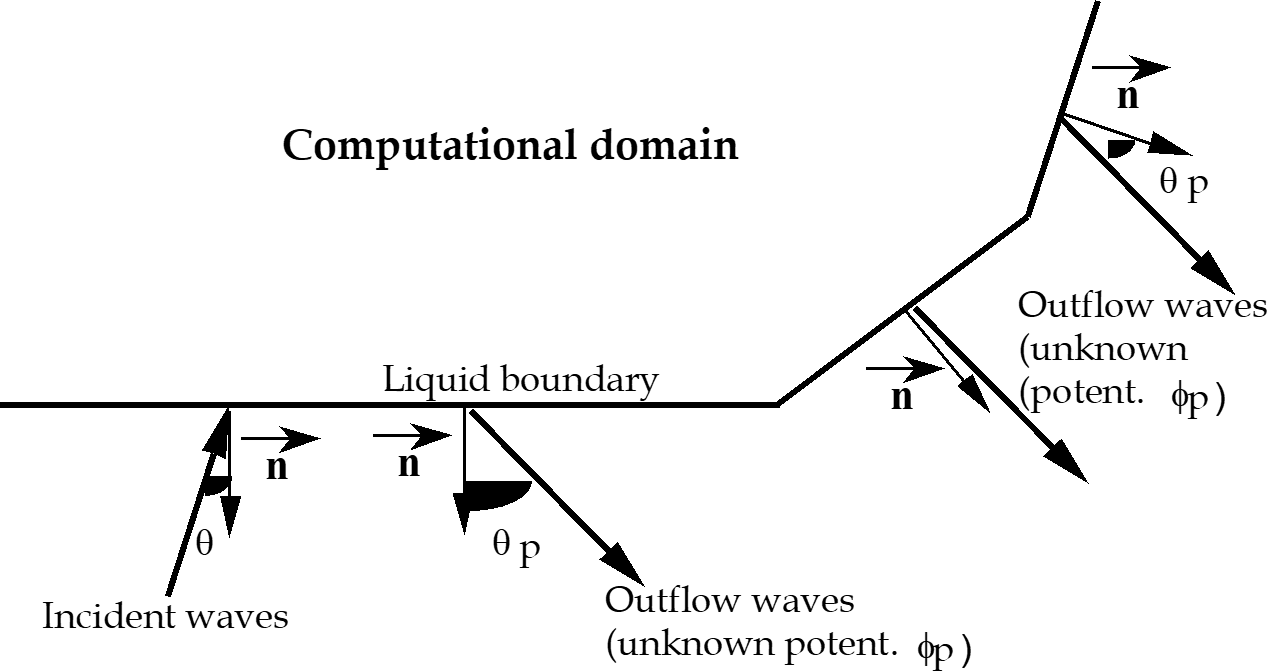
\includegraphics[width=\textwidth]{./graphics/incid_wave}
%
\caption{Illustration of incident wave boundaries}\label{fig:incid_wave}
\end{center}
\end{figure}

The potential $\gamma$ is user-specified by means of keywords and programming in
the BORH subroutine through the incident wave height and direction of
propagation. In case of a random wave computation, the incident wave height to
be specified is the \underbar{significant} height. On the other hand, the
monochromatic wave height values obtained using ARTEMIS are to be compared, as
required, with such data as energy height (H${}_{e}$) or rms height
(H${}_{rms}$) from random wave experiments. Angle $\theta_{p}$ is to be
specified as much as possible. In most cases $\theta_{p}$ is a priori unknown.
It is then recommended either to set $\theta_{p}$~=~0, or to make iterations
for assessing its value, as suggested in the previous paragraph. It would also
be possible to compute the difference $\phi - \gamma$ after an initial
computation giving a solution for $\phi$, and to derive the wave outflow angle
corresponding to that difference $\phi - \gamma$.


\paragraph{Free outflow}

In that case, $\gamma = 0$ and the boundary conditions is written as:

\begin{equation}
  \frac{\partial \phi}{\partial n} -ik\cos\theta_p \phi = 0
  \label{3.62}
\end{equation}

Once again, the angle $\theta_{p}$ is to be specified as best as possible, if
the wave outflow direction is known a priori (refer to the following Figure 5)
If no proper angle $\theta_{p}$ is specified, stray reflections contaminating
the computational domain from the boundary will predictably be noticed.


\begin{figure}[H]%
\begin{center}
%
  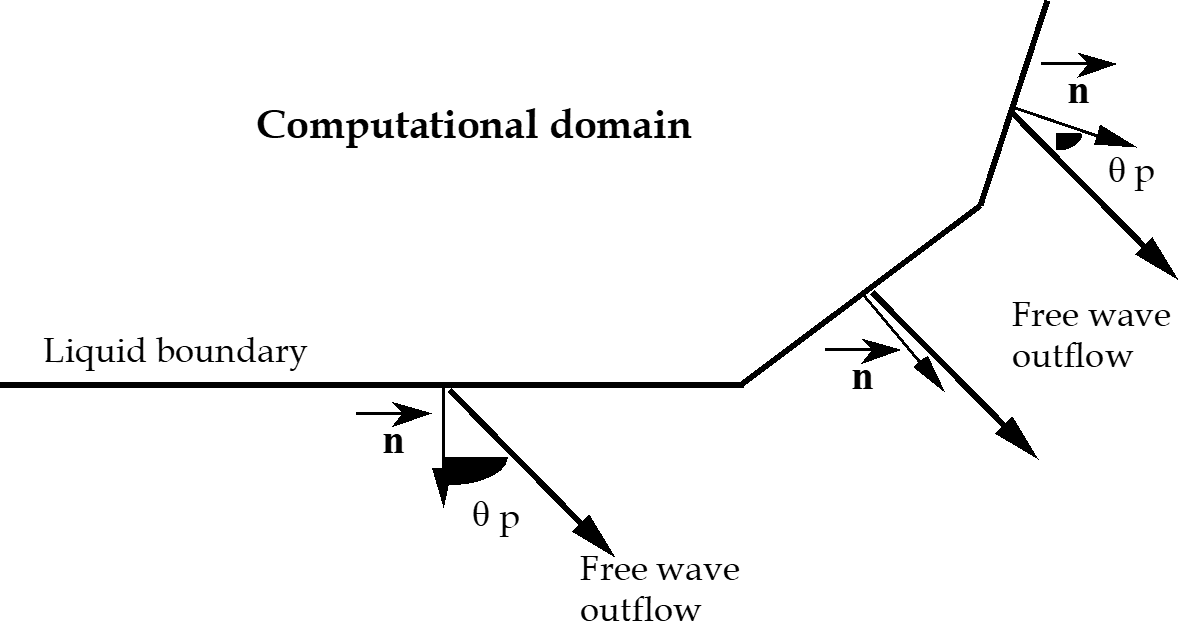
\includegraphics[width=\textwidth]{./graphics/free_outlaw}
%
\caption{Illustration of free outflow boundaries}\label{fig:free_outlaw}
\end{center}
\end{figure}


\section{Treatment of random mono/multi directional waves}\label{random_mono}

An actual wave exhibits a random feature when its energy is determined neither
by a single wave period or frequency nor by a single direction of propagation
(see in Section~\ref{waves}). It may be interpreted as the superposition of several
monodirectional waves with different periods and random lags in relation to
each other. The energy of an actual wave is the sum of monodirectional wave
energies making it up.

The waves whose frequencies range from f to f+df and whose directions of
propagation range from $\theta$ et $\theta$+d$\theta$, contribute to the total
energy (to within the term $\rho$g) up to S(f,$\theta$).df.d$\theta$ wherein
S(f,$\theta$) denotes the spectral density of variance as already introduced in
Section~\ref{spectral_appr}).

There are various formulations for expressing the spectral density of variance
according to the wave features. The most commonly used formulation was
developed from the JONSWAP campaign in the North sea~\ref{Hasselman}. It
assumes that the energy spectrum can be written in the form of the following
product:

\begin{equation}
  S(f,\theta) = J(f).G(\theta)
  \label{3.63}
\end{equation}

The frequency dependency J(f) is expressed by:

\begin{equation}
  J(f) = \delta H^2_s f_p^4 \text{exp}\left[-1.25\left(\frac{f_p}{f}\right)^4\right] \gamma^{\text{exp}\left[-0.5\left(\frac{f/f_p -1}{\alpha}\right)^2\right]}
  \label{3.64}
\end{equation}

wherein:
\begin{itemize}
  \item H${}_{s}$ is the significant wave height

  \item f${}_{p}$ is the peak frequency corresponding to the spectral maximum

  \item $\sigma$ is a dimensionless parameter which is determined as follows:

    \[
      \left\{
      \begin{matrix}
        \text{if } f \leq f_p \quad \sigma = 0.07\\
        \text{if } f > f_p \quad \sigma = 0.09
      \end{matrix}
      \right.
      \]

  \item $\gamma$ is a real number usually ranging from 1 to 7. The spectrum is
    called a Pierson-Moskowitz spectrum when the value is 1. Otherwise, it is
    called a JONSWAP spectrum. This parameter determines the spectral frequency
    spreading.

  \item $\delta$ is a weight coefficient that depends on $\gamma$:

    \[ \delta = \frac{0.0624}{0.230+0.0336\gamma-\frac{0.185}{1.9+\gamma}} \]

\end{itemize}


The trend of J(f) versus f/f${}_{p}$ is given in Fig~\ref{jonswap} for various values of $\gamma$.


\begin{figure}[H]%
\begin{center}
%
  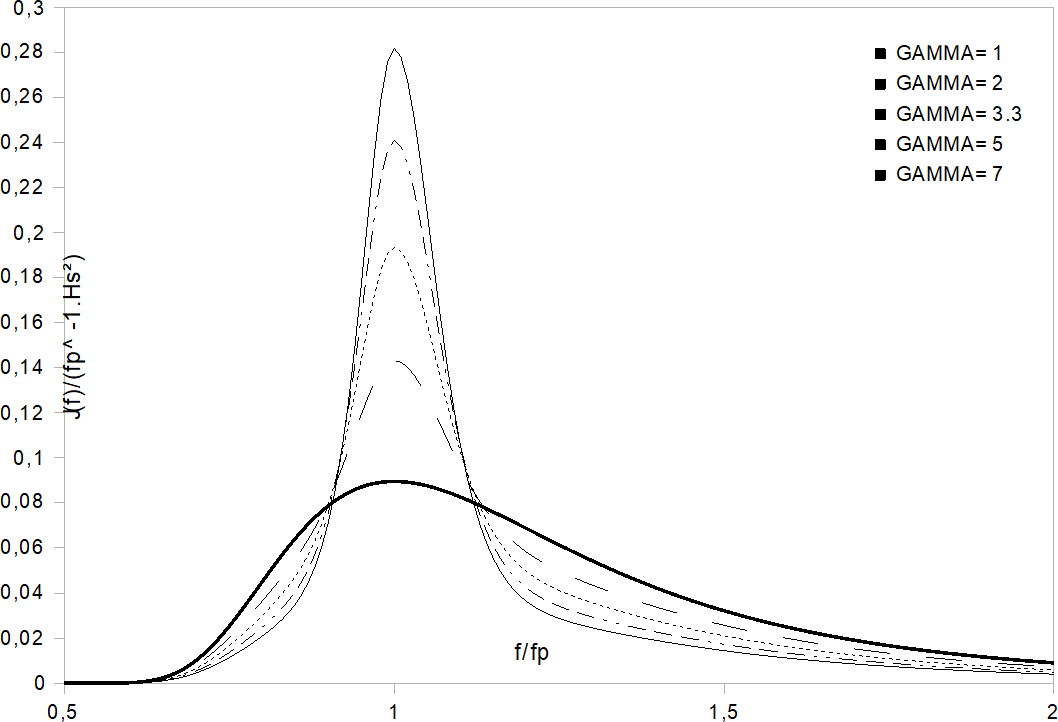
\includegraphics[width=\textwidth]{./graphics/jonswap}
%
\caption{Non dimensionnal theoretical JONSWAP spectrum}\label{fig:jonswap}
\end{center}
\end{figure}

The directional distribution G($\theta$) is often chosen in the following for
(refer to~\cite{Goda2000}):


\begin{equation}
  G = G_0 \cos^{2s}[(\theta-\theta_0)/2]
  \label{eq:3.65}
\end{equation}

wherein:
\begin{itemize}
  \item $\theta$ is the angle indicating the wave propagation direction

  \item $\theta_{0}$ denotes the main direction of wave propagation

  \item s is a positive real exponent of some tens (the higher s is, the less
    spread the directional spectrum is).

  \item G${}_{0}$ is a constant as determined by normalizing function G:

    \[ \int_{\theta_{min}}^{\theta^{max}}Gd\theta = 1  \]

  \item $\theta_{min}$ et $\theta_{max}$ indicate the boundary propagation
    directions of the waves being studied.

\end{itemize}

The trend of function G for various values of the coefficient "s" is described
in Fig.~\ref{fig:dir_dist}.

\begin{figure}[H]%
\begin{center}
%
  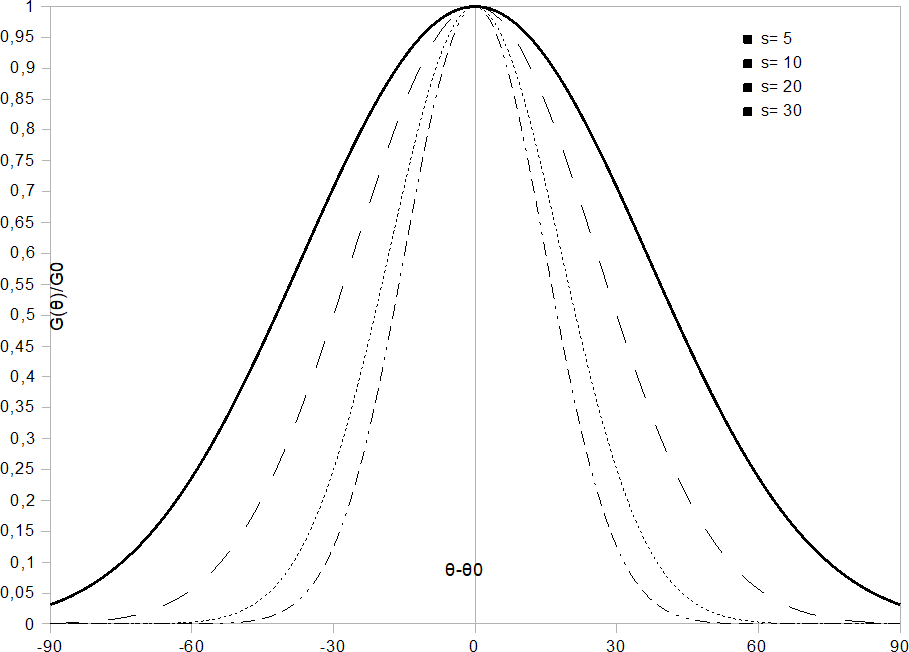
\includegraphics[width=\textwidth]{./graphics/dir_dist}
%
\caption{Directional distribution G($\theta$)}\label{fig:dir_dist}
\end{center}
\end{figure}

For \artemis{}, a random mono/multi-directional wave computation will consist
in discretizing the axes of the incident wave energy spectrum into a sequence
of values f${}_{i}$ for frequencies and $\theta_{j}$ for directions (1
$\mathrm{\le}$ i $\mathrm{\le}$ i${}_{max}$ and 1 $\mathrm{\le}$ j
$\mathrm{\le}$ i${}_{max}$), then making a steady wave computation for each of
these pairs by solving the mild-slope equation associated with the prescribed
boundary conditions, and lastly recombining the results for providing the
random wave features.

We have adopted a frequency and direction discretization of spectra which
divides each of the spectra into equal energy bands. Thus,
J($f_{i}$).$\Delta f_{i}$ and G($\theta_{j}$).$\Delta \theta_{j}$ are
constant for any i and j. The maximum values of i and j, i.e.\ i${}_{max}$ and
j${}_{max}$, are set by the user through keywords. The various steady wave
computations are then made with the same incident energy, the amount of which
is J(f${}_{i}$).$\Delta$f${}_{i}$.G($\theta_{j}$).$\Delta \theta_{j}$. It is
noteworthy that the constants being used in the expressions of J and G
(G${}_{0}$, H${}_{s}$\ldots) are purposeless for computing f${}_{i}$ and
$\theta_{j}$.

Frequency f${}_{i}$ denotes the i band in the J(f) spectrum. It is computed so
that f${}_{i}$ divides the i band into a couple of bands also of the same area.
Practically, when it is desired to cut the spectrum into i${}_{max}$ bands of
the same area, it is actually cut into 2i${}_{max}$ bands while systematically
recording the frequencies at the limits of these bands. The f${}_{i}$ values
are obtained taking the 2${}^{nd}$, 4${}^{th}${\dots} recorded frequencies. The
same procedure is applied to the directional spectrum G ($\theta$).

For each pair (f${}_{i}$, $\theta_{j}$), the model provides a significant wave
heightwave height H${}_{m0,k}$ ($1 < k < i_{max}j_{max}$) at each node of the
grid. Wave defined by (fi, $\theta$j) at a node of the grid contributes to the
total energy up to $\frac{1}{8}\rho g H^2_{e,k} = \frac{1}{4}\rho gH^2_{m_0, k}$, wherein $H_{e,k}$ and $H_{m_0 ,k}$ denote the
spectral energy height and significant height, respectively, as computed for
waves defined by (fi, $\theta$j).

The total incident energy is $\frac{1}{8}\rho g H^2_{e,inc}$ wherein $H_{e,inc}$
is the is the energy height of incident waves. Since each computation is made
with the same energy (the bands cutting the spectrum axes define the same
volume), He,inc is identical for all the computations. The total energy at a
point in the domain is:

\begin{equation}
  \frac{1}{8}\rho g \frac{1}{i_{max}.j_{max}}\sum_k H^2_{e,k}
  \label{3.66}
\end{equation}

The resulting energy height $H_e$ is derived there from at each node of the
grid:

\begin{equation}
  H_e = \sqrt{\frac{1}{i_{max}.j_{max}}\sum_k H^2_{e,k}}
  \label{3.67}
\end{equation}

The significant wave height $H_{m_0}$ can be derived from the energy height
$H_{e}$ through the relation mentioned in Section~\ref{spectral_appr}:

\[ H_{m_0} = \sqrt{2}H_e\]


That quantity is retrieved by \artemis{} in the case of random wavesrandom
waves. Assuming that the distribution of wave heights follows a Rayleigh's law,
the spectral and statistical coefficients, i.e (H${}_{m_0}$ ;
H${}_{e}$) on the one hand and (H${}_{1/3}$ ; H${}_{rms}$) on the other hand,
respectively, are equivalent to one another.


\section{Radiation stresses; Wave-driven forcing terms}

Both in monochromatic and random modes, \artemis{} enables to compute the
radiation stresses Sxx, Sxy and Syy, from the general following
equation~\cite{Dingemans1987}
\[S_{ij} =\frac{E}{2} \left[\frac{k_{i} k_{j} }{k^{2} } \frac{2C_{g} }{C} +\left(\frac{2C_{g} }{C} -1\right)\; \delta _{ij} \right]\]

 with:

\begin{itemize}
\item  $E=\frac{1}{8} \rho gH_{e}^{2} $  (H${}_{e}$ is the energetic wave height)

\item  indexes i and j correspond to x or y
\end{itemize}

In regular mode (monochromatic wave), the energetic wave height
H${}_{e}$ is the wave height directly given by \artemis{}. In random mode,
this wave height H${}_{e}$ is roughly proportional to the
significant wave height:$H_{e} \approx H_{s} /\sqrt{2} $. Other parameters
involved in the previous general equation correspond to the mean values defined
in the table given above: mean wave number, mean celerities\ldots

We can deduce from these radiation stresses the associated forcing F${}_{x}$ and F${}_{y}$ to be introduced in a current model (for instance TELEMAC-2D), which will be able to compute the wave-driven currents. These forcing terms are expressed as follows:
\[F_{x} =-\frac{1}{h} \left(\frac{\partial S_{xx} }{\partial x} +\frac{\partial S_{xy} }{\partial y} \right)\]
\[F_{y} =-\frac{1}{h} \left(\frac{\partial S_{xy} }{\partial x} +\frac{\partial S_{yy} }{\partial y} \right)\]

  with: h the water depth at rest

\underbar{Remark 1}: Simulation of the wave-driven currents with the TELEMAC-2D software is performed through an external coupling between \artemis{} and TELEMAC-2D.

\underbar{Remark 2}: in the monochromatic mode, oscillations are often observed on the wave heights results. They may be generated by (i) real reflections against solid obstacles which propagate within the computational domain, or by (ii) undesired reflections due to boundary conditions problems. These undesired reflections may greatly alter the computation of the wave forcing terms. To avoid this problem, it is possible in release 6, for the monochromatic mode, to impose an automatic smoothing of the wave heights field, in order to filter these oscillations, whose characteristic « wave » length is half the « wave » length of the waves. To achieve this smoothing, one has to activate the new key-word:

WAVE HEIGHTS SMOOTHING

whose mnemonic is LISHOU (default value : NO).

\textbf{However, it is preferable to use \artemis{} in random mode to get satisfactory estimation of the wave forcing terms}


\section{Digital solution through the finite element method}\label{digi_sol}


\subsection{System of equations to be solved}

The differential system to be solved, the unknown of which is the reduced
potential $\phi$, comprises the amended mild-slope equation as well as
equations expressing the boundary conditions at each boundary of the
computational domain.

\begin{equation}
  \phi(x,y) = \phi_r (x,y) +i\phi_i (x,y)
  \label{eq:3.68}
\end{equation}

$\phi_{r}$ and $\phi_{i}$ being real functions depending on x and y, which are
the real and imaginary components of $\phi$, respectively. That function $\phi$
will hereinafter be termed the potential by misuse of language, though
multiplying it by $f(z)e^{-\omega t}$ is required for getting the total potential $\Phi$.

The differential system to be solved is then as follows:

\begin{equation}
  \left\{
  \begin{matrix}
    \nabla.(CC_g \nabla\phi)+CC_g(k^2+ik\mu)\phi = 0 & \\
    \text{and according to the boundary conditions} & \\
    \frac{\partial \phi}{\partial n} -i\frac{1-Re^{i\omega}}{1+Re^{i\omega}}k\cos\theta_p \phi = 0 \quad & \text{(solid wall)} \\
    \frac{\partial \phi}{\partial n} -ik\cos\theta_p \phi = \frac{\partial \gamma}{\partial n}-ikcos\theta_p \gamma \quad & \text{(incident wave)} \\
    \frac{\partial \phi}{\partial n} -ik\cos\theta_p \phi = 0 \quad & \text{(free outflow)}
  \end{matrix}
  \right.
  \label{eq:3.69}
\end{equation}


\subsection{Variational formulation of the problem}

The mild-slope equation is elliptical and can only be solved through the finite
element method. The differential system~\ref{eq;3.69} to be solved is
then transformed through a variational formulation of the problem.

If $\Omega$ is the computational domain, $\Gamma$ its boundary and if
$\Psi$ denotes a basic function of class C${}_{1}$ on $\Omega$, the variational
formulation of the mild-slope equation is expressed as :

\begin{equation}
  \forall \psi \in C_1(\Omega), \int_{\Omega}\Psi[\nabla.(CC_g\nabla\phi)+CC_g(k^2+ik\mu)\phi]\text{d}\Omega = 0
  \label{eq:3.70}
\end{equation}

Due to the properties of $\psi$, integration in parts is possible :

\begin{equation}
  \int_{\Gamma}\Psi CC_g \frac{\partial \phi}{\partial n}\text{d}\Gamma - \int_{\Omega}CC_g\nabla\Psi.\nabla\phi \text{d}\Omega+\int_{\Omega}CC_g(k^2+ik\mu)\Psi\phi \text{d}\Omega = 0
  \label{eq:3.71}
\end{equation}

The normal derivative of the potential at the boundary $\Gamma$ of the domain
will then come out. It can be replaced by its expression as given by the
boundary conditions, which is in the following form:

\begin{equation}
  \frac{\partial \phi}{\partial n} = (A\phi_i + B\phi_r) + i(-A\phi_r+B\phi_i) -E -iF
  \label{eq:3.72}
\end{equation}

wherein A, B, E and F are real numbers determined by the kinds of boundary
conditions as specified in all the parts of $\Gamma$.

The following system can be achieved by separating the real and imaginary parts:

\begin{equation}
  \left\{
    \begin{matrix}
      \int_{\Gamma}\Psi CC_g(B\phi_r + A\phi_i)\text{d}\Gamma -\int_{\Omega}CC_g\nabla\Psi.\nabla\phi_r \text{d}\Omega \\
      \quad +\int_\Omega CC_g\Psi(k^2\phi_r -k\mu\phi_i)\text{d}\Omega = \int_\Gamma\Psi CC_g E \text{d}\Gamma \\

      \int_{\Gamma}\Psi CC_g(-A\phi_r + B\phi_i)\text{d}\Gamma -\int_{\Omega}CC_g\nabla\Psi.\nabla\phi_i \text{d}\Omega \\
      \quad +\int_\Omega CC_g\Psi(k^2\phi_i -k\mu\phi_r)\text{d}\Omega = \int_\Gamma\Psi CC_g F \text{d}\Gamma \\
    \end{matrix}
    \right.
  \label{eq:3.73}
\end{equation}


\subsection{Digital solution algorithm}

\paragraph{Discretization. Setting into a matrix form}

Linear basic functions are chosen on triangular elements. These functions are
really  functions of class C${}_{1}$. $\phi_r$ and $\phi_i$ are resolved on
these basic functions.
\begin{equation}
\left\{
  \begin{matrix}
  \phi_r =\sum_{j=1}^{\text{NPOIN}} \phi_r^j\Psi_j^e \\
  \phi_i =\sum_{j=1}^{\text{NPOIN}} \phi_i^j\Psi_j^e \\
  \end{matrix}
  \right.%
  \label{eq:3.74}
\end{equation}
NPOIN is the total number of points in the grid. The $\psi_{j}^{e}$
functions are linear at each element with an e index and are null everywhere
else.

By incorporating these expressions into the previously described set of
equations, a matrix system can be obtained in the following form:

\begin{equation}
  \left(
  \begin{matrix}
    \text{AM} & \text{BM} \\
    -\text{BM} & \text{AM}
  \end{matrix}
  \right).
  \left(
    \begin{matrix}
     \phi_r \\
     \phi_i
    \end{matrix}
  \right) =
  \left(
  \begin{matrix}
    \text{CV1} \\
    \text{CV2}
  \end{matrix}
  \right)
  \label{eq:3.75}
\end{equation}

In order to obtain a positive diagonal along AM (the reason for it will be
explained later), the couple of previous equations have multiplied by -1. AM is
a matrix provided with NPOIN x NPOIN dimensions and having as a general term:

\begin{equation}
  AM_{jk} = -\int_\Gamma \Psi_j \Psi_k CC_g B \text{d}\Gamma +
             \int_\Omega CC_g \nabla\Psi_j.\nabla\Psi_k d\Omega +
             \int_\Omega CC_g k^2 \Psi_j \Psi_k d\Omega
  \label{eq:3.76}
\end{equation}

BM is also a NPOIN x NPOIN-dimensioned matrix having as a general term:

\begin{equation}
  BM_{jk} = -\int_\Gamma \Psi_j \Psi_k CC_g A \text{d}\Gamma +
             \int_\Omega \Psi_j \Psi_k CC_g k\mu d\Omega
  \label{eq:3.77}
\end{equation}

$\phi_{r}$ and $\phi_{i}$ are a couple of NPOIN-dimensioned vectors comprising  components.

CV1 and CV2 are a couple of vectors that are null everywhere but at the edge of
the grid. The NPTFR-dimensioned edge vectors have the following general terms:

\begin{equation}
  \begin{matrix}
  \text{CV1} = -\int_\Gamma \Psi_k CC_g E \text{d} \Gamma \\
  \text{CV2} = -\int_\Gamma \Psi_k CC_g F \text{d} \Gamma
  \end{matrix}
  \label{eq:3.78}
\end{equation}

If the diagonal term in the AM matrix is positive, a suitable preconditioning
will become applicable to the system, what will make the resolution much
faster. Regardless of the edge term, AM${}_{jk}$ has approximately the sign of $1/(\Delta x)^2-k^2$
($\Delta$x denoting the mean size of the meshes). As long as
1/($\Delta$x)~$\mathrm{>}$~k, i.e.\ as long as $\Delta$x~$\mathrm{<}$~L/2$\pi$,
the diagonal term remains positive. Due to that condition, the selected mesh
size shall be smaller than L/7. It seems that at least 7 grid nodes per
wavelength are required.

In simple examples, however, we have tested coarser grids having 4-5 nodes per
wavelength. The results for these computational conditions remain satisfactory
even though, in such a case, no preconditioning is applied to the matrix
system. With less than 4 nodes per wavelength, the spatial resolution is too
low and the information is deteriorated.


\paragraph{Computing the matrices}

The AM and BM matrices as well as the CV1 and CV2 members are computed by the
subroutines of the finite element library BIEF~\cite{Hervouet2006}. These
matrices are computed for one element at a time. Only their diagonals are put
together. For assisting computations, we have taken the product CC${}_{g}$ with
P1 discretization on each of the triangles. The coefficients A, B, E and F are
taken as constants on each of the edge segments (P0 discretization).

C and C${}_{g}$ are computed from the wave number k as obtained through the
Airy's dispersion relation:

\begin{equation}
  \frac{\omega^2}{gk} = th(kh)
  \label{eq:3.79}
\end{equation}

Taking x = kh and y = , the dispersion relation becomes y = xth(x). A precise, explicit form of it is used at 0.5 10${}^{-3\ }$:
\begin{equation} \label{GrindEQ__3_80_}
{\rm x}=\sqrt{{\rm y}} {\rm \; }\left({\rm y+}\frac{{\rm 1}}{{\rm 1+}\mathop{{\rm \Sigma \; }}\limits_{{\rm j=1}}^{{\rm 5}} {\rm p}_{{\rm j}} {\rm y}^{{\rm j}} } {\rm \; }\right)^{\frac{{\rm 1}}{{\rm 2}} } {\rm \; \; \; avec\; }\left\{\begin{array}{l} {{\rm p}_{{\rm 1}} {\rm =0.6522}} \\ {{\rm p}_{{\rm 2}} {\rm =0.4622}} \\ {{\rm p}_{{\rm 3}} {\rm =0.}} \\ {{\rm p}_{{\rm 4}} {\rm =0.0864}} \\ {{\rm p}_{{\rm 5}} {\rm =0.0675}} \end{array}\right.
\end{equation}


\paragraph{Solution of linear system}

The dissipation process is taken into account by a new term in the BM matrix.
That term is related to a dissipation coefficient $\mu$ which is explained in
Section~\ref{dissipation_coeff} depending on whether either or both of
breaking and bottom friction are considered. The difficulty lies in that $\mu$
always depends on H, i.e.\ on the unknown quantity $\phi$in the problem. Thus,
the linear system cannot be solved directly. The solution that was adopted is a
prediction-correction scheme. A first assessment of the coefficient $\mu$ is
made throughout the computational domain. The linear system is then solved
though one of the methods as proposed in the BIEF library of the TELEMAC system

\begin{itemize}
\item  Either using an iterative method: conjugate gradient, conjugate gradient
  on normal equation, GMRES solver\ldots~\cite{Hervouet2006};

\item  Or using the direct solver.
\end{itemize}

A first solution $\phi_{1}$ is obtained. It makes it possible to compute a
second assessment of dissipation $\mu_{2}$. That second assessment is used for
solving again the linear system and obtaining a solution $\phi_{2}$. The
process is interrupted when the user thinks that the difference between the two
successive solutions is sufficient or when the number of such repeated
subiterations has reached a boundary value which is also set by the user. A
sub-relaxation was prescribed for that process in order to assist the
convergence of the method. That relaxation coefficient is specified by the
user..

The overall solution algorithm is summarised in the diagram below:

\begin{figure}[H]%
\begin{center}
%
  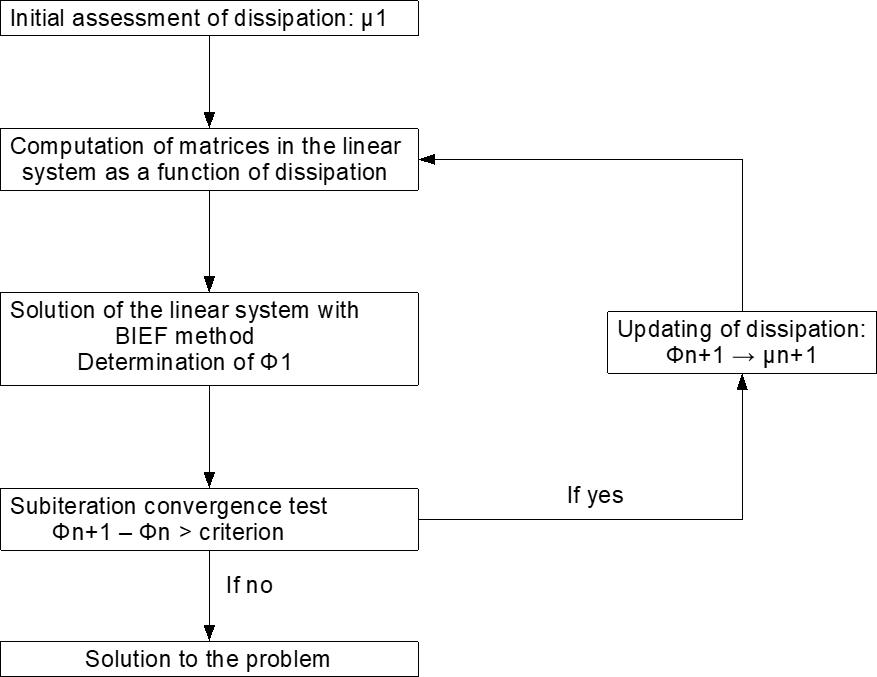
\includegraphics[width=\textwidth]{./graphics/dissipation}
%
\caption{Directional distribution G($\theta$)}\label{fig:dissipation}
\end{center}
\end{figure}

%TODO: Reference to reference manual
It seems that the most suitable iterative resolver for the linear system being
considered is the direct solveur. That resolver is taken by default by the
model. The matrix may previously be diagonally preconditioned. The user,
however, may freely choose any other resolver and any other preconditioning as
proposed through keywords in BIEF (see in {\S} 9).

As regards random waves, the previously described algorithm will be followed as
many times as necessary because of the energy spectrum discretization (i.e.\
i${}_{max}$*j${}_{max}$ times). In order to improve the wave computation time
corresponding to the pairs (f${}_{i+1}$, $\theta_{j}$), (f${}_{i}$,
$\theta_{j+1}$), and (f${}_{i+1}$, $\theta_{j+1}$), however, those values which
were previously computed for the pair (f${}_{i}$, $\theta_{j}$) are used for
initializing the unknowns and the dissipation coefficient.

Practically, it appears that the number of iterations implied by the resolver
convergence is substantially the same as the number of nodes in the NPOIN grid.
Since the required time for an iteration (consisting in a product of a matrix
by a vector) is proportional to the number of nodes, the time for a computation
by \artemis{} is globally proportional to the square of the number of nodes.
The proportionality coefficient depends, among others, on the king of
computational domain boundaries, on bathymetry and on the computing machine.
The more numerous the liquid boundaries are, the smaller it is. The greater the
depths are, the higher it is. This is because, as it is well known, a diffusion
matrix can more hardly be inverted than a mass matrix. Now, the greater the
depth is, the higher the phase and group velocities are. The diffusion matrix
then becomes increasingly prevailing in relation to the mass matrix. The
required number of sub-iterations for providing the convergence of the
computation of the dissipation terms is usually 4 or 5.


\subsection{Matrix in the case of rapidly varying topography}

Here we explain how rapidly variying topoghrapy is computed, and how the
extended mild-slope equation is taken into account.


\paragraph{Variational formulation of the problem}


With the same idea we used in 2.8.2 (wrong link), the variational formulation
becomes for a basic function $\psi$ (C1):
\[\int _{\Omega }\psi \cdot \left\{\nabla \left(CC_{g} \cdot \nabla \phi \right)+CC_{g} \left(k^{2} \cdot \left(1+f\right)+ik\mu \right)\phi \right\} d\Omega =0\]
An integration in parts gives :
\[\int _{\Gamma }\psi \cdot CC_{g} \cdot \frac{\partial \phi }{\partial n} \cdot  d\Gamma -\int _{\Omega }CC_{g} \cdot \nabla \phi \cdot \nabla \psi \cdot  d\Omega +\int _{\Omega }CC_{g} \left(k^{2} \cdot \left(1+f\right)+ik\mu \right)\cdot \phi \cdot \psi \cdot  d\Omega =0\]
The boundary conditions can be expressed as :
\[\frac{\partial \phi }{\partial n} =\left(A\phi _{i} +B\phi _{r} \right)+i\cdot \left(-A\phi _{r} +B\phi _{i} \right)-E-iF\]
Separating imaginary and real parts (f is real) :
\[\int _{\Gamma }\psi \cdot CC_{g} \cdot \left(B\phi _{r} +A\phi _{i} \right)\cdot  d\Gamma -\int _{\Omega }CC_{g} \cdot \nabla \phi _{r} \cdot \nabla \psi \cdot  d\Omega +\int _{\Omega }CC_{g} \left(k^{2} \cdot \left(1+f\right)\cdot \phi _{r} -k\mu \cdot \phi _{i} \right)\cdot \psi \cdot  d\Omega =\int _{\Gamma }\psi \cdot CC_{g} \cdot E\cdot  d\Gamma \]
\[\int _{\Gamma }\psi \cdot CC_{g} \cdot \left(-A\phi _{r} +B\phi _{i} \right)\cdot  d\Gamma -\int _{\Omega }CC_{g} \cdot \nabla \phi _{i} \cdot \nabla \psi \cdot  d\Omega +\int _{\Omega }CC_{g} \left(k^{2} \cdot \left(1+f\right)\cdot \phi _{i} -k\mu \cdot \phi _{r} \right)\cdot \psi \cdot  d\Omega =\int _{\Gamma }\psi \cdot CC_{g} \cdot F\cdot  d\Gamma \]


\paragraph{Matrix}

Matrix AM, expressed in~\ref{eq:3.76} is modified. BM doesn't change and the
second member (CV1 and CV2) is unchanged too.
\[AM_{jk} =\int _{\Gamma }\psi _{j} \psi _{k} \cdot CC_{g} \cdot B\cdot  d\Gamma -\int _{\Omega }CC_{g} \cdot \nabla \psi _{j} \cdot \nabla \psi _{k} \cdot  d\Omega +\int _{\Omega }CC_{g} \cdot k^{2} \cdot \left(1+f\right)\cdot \psi _{j} \cdot \psi _{k} \cdot  d\Omega \]


\paragraph{Computation and implementation}

The user include the keyword «RAPIDLY VARYING TOPOGRAPHY~» in the case file.
This keyword can take the value 0, 1, 2 or 3.Default value is 0.

\begin{itemize}
  \item 0: correspond to classical mild-slope equation.

  \item 1: gradient effects are taken into account.

  \item 2: curvature effects are taken into account.

  \item 3: both gradient and curvature effects are taken into account.
\end{itemize}

This value is red in the BERKHO routine. Is the value is different from 0
routine PENTCO is called. In PENTCO we compute the term «~f~» in the whole
domain. Depending on the user's choice, Matrix AM is modified in BERKHO.

To get the value of «~f~», PENTCO calls to functions:

FCTE1.f, for gradient terms:
\[E_{1} \left(kh\right)=\frac{\left\{x^{4} +4x^{3} \sinh (x)-9\sinh (x)\sinh (2x)+3x\left(x+2\sinh (x)\right)\cdot \left(\cosh ^{2} (x)-2\cosh (x)+3\right)\right\}}{3\left(x+\sinh (x)\right)^{4} } \]
With $x=2kh$

If x is too small (lower \`{a} 10-3), the value of the function is simply:
\[E_{1} \left(kh\right)=-1/6\]
FCTE2.f,  for curvature terms.

$\tilde{E}_{2} \left(kh\right)=\frac{\left\{\tanh (x)-x\right\}\cdot \cosh (x)}{x\cdot \left(x+\sinh (x)\right)^{2} } $

If x is too small (lower \`{a} 10-3), the value of the function is simply:

$\tilde{E}_{2} \left(kh\right)=-1/12$

We note that
\[\frac{E_{2} \left(kh\right)}{k_{0} } =2h\cdot \tilde{E}_{2} \left(kh\right)\]
At the end, PENTCO computes:

\begin{itemize}
\item  RAPIDLY VARYING TOPOGRAPHY = 1
\[f=E_{1} (kh)\cdot \left(\nabla h\right)^{2} \]

\item  RAPIDLY VARYING TOPOGRAPHY = 2
\[f=2h\cdot \tilde{E}_{2} (kh)\cdot \Delta h\]

\item  RAPIDLY VARYING TOPOGRAPHY = 3
\[f=E_{1} (kh)\cdot \left(\nabla h\right)^{2} +2h\cdot \tilde{E}_{2} (kh)\cdot \Delta h\]
\end{itemize}


In any other case, the value of f is 0.

\eject


\chapter{Inputs and outputs}


\section{Preliminary remarks}

During a computation, the \artemis{} software uses a number of input and output files, some of which are optional.

The input files are the following:

\begin{itemize}
\item  The geometry file

\item  The steering file

\item  The boundary conditions file

\item  The bottom topography file

\item  The FORTRAN file

\item  The binary data files

\item  The formatted data files
\end{itemize}

The output files are the following:

\begin{itemize}
\item  The results file

\item  The printout listing

\item  The formatted data file

\item  The binary data file
\end{itemize}


\section{The files}


\subsection{The steering file}

This is a text file created by FUDAA-PREPRO or directly by the text editor. In
a way, it represents the control panel of the computation. It contains a number
of keywords to which values are assigned. If a keyword is not contained in this
file, \artemis{} will assign it the default value defined in the dictionary
file. If such a default value is
not defined in the dictionary file, the computation will stop with an error
message. For example, the command "wave period=10." enables the user to specify
that the wave period is 10 seconds.

\artemis{} reads the steering file at the beginning of the computation.

The dictionary file and steering file are read by a utility called
DAMOCLES, which is included in \artemis{}\@. Because of this, when
the steering file is being created, it is necessary to comply with
the rules of syntax used in DAMOCLES (this is done automatically if the file is
created with FUDAA-PREPRO). They are briefly described below and an example is
given in Appendix 8.

The rules of syntax are the following:

\begin{itemize}
\item  The keywords may be of Integer, Real, Logical or Character type.

\item  The order of keywords in the steering file is of no importance.

\item  Each line is limited to 72 characters. However, it is possible to pass from one line to the next as often as required, provided that the name of the keyword is not split between two lines.

\item  The signs ":" or "=" can be used indiscriminately as separator for the name of a keyword and its value. They may be preceded or followed by any number of spaces. The value itself may appear on the next line. For example:
\end{itemize}

\telkey{wave period = 10.}

or

\telkey{WAVE PERIOD: 10.}

or again

\telkey{WAVE PERIOD =10.}

\begin{itemize}
\item  Characters between two "/" on a line are considered as comments. Similarly, characters between a "/" and the end of line are also considered as comments. For example:
\end{itemize}

\telkey{SOLVER = 3 / Conjugated gradient on normal equation}

\begin{itemize}
\item  A line beginning with "/" is considered to be all comment, even if there is another "/" in the line. For example:
\end{itemize}

/ The geometry file is "./mesh/geo"

\begin{itemize}
\item  A line beginning with "/" is considered to be all comment, even if there is another "/" in the line. For example:
\end{itemize}

/ The geometry file is "./mesh/geo"

\begin{itemize}
\item  When writing integers, do not exceed the maximum size permitted by the
  computer (for a computer with 32-bit architecture, the extreme values are -2
    147 483 647 to + 2 147 483 648. Do not leave any space between the sign
    (optional for the +) and number. A full stop is allowed at the end of a
    number.

\item  When writing real numbers, the full stop and comma are accepted as
  decimal points, as are E and D formats of FORTRAN. ( 1.E-3 0.001 0,001 1.D-3
    represent the same value).

\item  When writing logical values, the following are acceptable: 1 \verb!OUI!
  \verb!YES! \verb!.TRUE.! \verb!TRUE! \verb!VRAI! and \verb!0! \verb!NON!
    \verb!NO! \verb!.FALSE.! \verb!FALSE! \verb!FAUX!.

\item  Character strings including spaces or reserved symbols ("/",":", "=",
  "\&") must be placed between apostrophes ('). The value of a character
    keyword can contain up to 144 characters. As in FORTRAN, apostrophes in a
    string must be doubled. A string cannot begin or end with a space. For
    example :
\end{itemize}

\telkey{TITLE = \''CAS DE L\''\''EPI\''}

In addition to keywords, a number of instructions or meta-commands interpreted during sequential reading of the steering file can also be used:

\begin{itemize}
\item  Command \telkey{\&FIN} indicates the end of the file (even if the file
  is not finished). This means that certain keywords can be deactivated simply
    by placing them behind this command in order to reactivate them easily
    later on. However, the computation continues.

\item  Command \telkey{\&ETA} prints the list of keywords and the value that is
  assigned to them when DAMOCLES encounters the command. This will be displayed
    at the beginning of the printout listing (see Section~\ref{listing}).

\item  Command \telkey{\&LIS} prints the list of keywords. This will be
  displayed at the beginning of the printout listing (see Section~\ref{listing}).

\item  Command \telkey{\&IND} prints a detailed list of keywords. This will be
  displayed at the beginning of the printout listing (see Section~\ref{listing}).

\item  Command \telkey{\&STO} stops the program and the computation is
  interrupted.

\item  The name of this file is given by using the keyword:\telkey{STEERING
  FILE.}
\end{itemize}


\subsection{The geometry file}

It is a SELAFIN-formatted binary file which can then be read by RUBENS or
FUDAA-PREPRO and is generated either by the MATISSE software or by the
\stbtel{} module (from the file(s) originating from of mesh generator). The
SELAFIN format structure is described in Appendix 11.

This file contains all the information concerning the mesh, i.e.\ the number of
mesh points (NPOIN variable), the number of elements (NELEM variable), the
number of nodes per element (NDP variable), arrays X and Y containing the
coordinates of all the nodes and array IKLE containing the table of
connectivities.

This file can also contain bottom topography information at each mesh point, if
such bottom topography has been interpolated during the running of module
\stbtel{} (for more information, see the User's Manual for this software).

ARTEMIS stores information on the geometry at the start of the results file.
Because of this, the computation results file can be used as a geometry file if
a new simulation is to be run on the same mesh.

The name of this file is given with the keyword: \telkey{GEOMETRY FILE}

In order to reach a good accuracy, it is necessary to build a mesh using at
least 3 points by wave length. In addition, during the numerical treatments, a
mesh with 7 points by wave length leads to matrices with non zero diagonals
that allows the use of preconditioning in order to improve the computation
speed.

When using random waves, a good method is to build a mesh using 7 points by
wave length for the peak period. When considering the lowest period, the
preconditioning will be probably not usable, but the refinement of the mesh
will not be under the criteria of 3 points by wave length.


\subsection{The boundary conditions file}

This is a formatted file generated automatically by \stbtel{}. It can be
modified with a standard text editor. Each line of the file is dedicated to one
point on the mesh boundary. The numbering used for points on the boundary is
that of the file lines. First of all, it describes the contour of the domain
trigonometrically, starting from the bottom left-hand corner (X + Y minimum)
and then the islands in a clockwise direction.

See Section~\ref{bnd_cond} for a fuller description of this file.

The file name is given with the keyword:\telkey{BOUNDARY CONDITIONS FILE}.

\subsection{The results file}

This is the file in which \artemis{} stores information during the computation.
It is normally in Selafin format. It contains first of all information on the
mesh geometry, then the names of the stored variables. It then contains the
period for each computed period and the values of the different variables for
all mesh points.

Its content is dependent on the value of the following keywords:

\begin{itemize}
\item  \telkey{GRAPHIC PRINTOUT PERIOD}: fixes the period for outputs when
  using computation over multiple periods (for example, case of period scanning
    to search resonance period).

\item  \telkey{VARIABLES FOR GRAPHIC PRINTOUTS} : this is used to specify the
  list of variables to be stored in the results file. Each variable is
    identified by an identifier (string with up to 8 characters); these are
    listed in Appendix 4 with the description of this keyword.
\end{itemize}

The name of this file is given with the keyword: \telkey{RESULTS FILE}


\subsection{The printout listing}\label{listing}

This is a formatted file created by \artemis{} during the computation. It
contains a report on the execution of ARTEMIS\@. Its content varies in
accordance with the values of the following keywords:

\begin{itemize}
\item  \textit{LISTING PRINTOUT PERIOD} : this fixes the period between two
  periods output when calculating several wave periods (period scanning). The
    given value is the number of periods. For example, the following sequence:
\end{itemize}

\telkey{LISTING PRINTOUT PERIOD = 2}

will produce a listing printout every 2 wave periods. Moreover, irrespective of
the period indicated by the user, the last period is systematically printed.

\begin{itemize}
\item  \textit{LISTING PRINTOUT}: this cancels the listing printout if the
  value is NO (the listing printout then only contains the program heading and
    normal end indication). However, this is not advisable in any
    circumstances.

\item  \textit{VARIABLES TO BE PRINTED} : this is used to specify the list of
  variables for which all values will be printed at each mesh point. This is a
    debugging option offered by ARTEMIS that should be handled with caution so
    as to avoid creating an excessively large listing printout.

\item  \textit{INFORMATION ABOUT SOLVER}: if this is required, at each printed
  period the user will have the number of iterations necessary to achieve the
    accuracy required during the mild slope equation calculation, or by default
    that reached at the end of the maximum number of iterations authorised. In
    addition, the user will obtain the number of sub-iterations necessary to
    take into account the dissipation phenomena.
\end{itemize}

The name of this file is managed directly by the \artemis{} start-up procedure.
In general, it has the name of the steering file associated with
the suffix ".sortie". A short example of a listing printout is given in Appendix
10.


\subsection{The Fortran user file}

The FORTRAN file contains all the \artemis{} subroutines modified by the user
and those that have been specially developed for the computation.

This file is compiled and linked so as to generate the executable program for
the simulation.

The name of this file is given with the keyword:\textit{FORTRAN FILE}

An example of a FORTRAN file is given in Appendix 9.


\subsection{The ancillary files}

Other files may be used by \artemis{}.

\begin{itemize}
\item  One or two binary data files, specified by the keywords
  \textit{BINARY DATA FILE 1} and \textit{BINARY DATA FILE 2}. These files can
    be used to provide data to the
    program, data reading being of course managed by the user within the
    Fortran program. The logical units affected to this two files are
    respectively 24 and 25.

\item  One or two formatted data files, specified by the keywords
  \textit{FORMATTED DATA FILE 1} and \textit{FORMATTED DATA FILE 2}. These
    files can be used to provide data to the program, data reading being of
    course managed by the user within the Fortran program. The logical units
    affected to this two files are respectively 26 and 27.

\item  A binary results file specified by the keyword \textit{BINARY RESULTS
  FILE}. This file can be used to store additional results. Write operations on
    the file are managed by the user in the Fortran program. The logical units
    affected to this file is 28.

\item  A formatted results file specified by the keyword \textit{FORMATTED
  RESULTS FILE}. This file can be used to store additional results. Write
    operations on the file are managed by the user in the Fortran program. The
    logical units affected to this file is 29.
\end{itemize}

Read and write operations on these files must be managed completely by the
user. Management can be done from any point accessible to the user. For
example, using a file to provide the initial conditions will mean managing it
with the subroutine CONDIH\@. Similarly, using a file to introduce boundary
conditions can be done in the BORH subroutine.


\subsection{The dictionary file}

This file contains all information on the keywords (name in French, name in
English, default values, type, documentation on keyword, information required
by FUDAA-PREPRO). This file can be consulted by the user but must under no
circumstances be modified.


\subsection{The libraries}

When a computation is started, the main program written by the user is compiled
and then linked to standard libraries in order to generate the program that is
then run.

During the link phase, the following libraries are used:

\begin{itemize}
\item  Library \artemis{}: this library contains the subroutines that are
  specific to the ARTEMIS computation code.

\item  Library bief: this library contains all the computation modules
  concerning operations of the finite-element type (operations on matrices and
    vectors). It is common to all the simulation codes developed by the
    Laboratoire National d'Hydraulique within the TELEMAC structure
    (``bief'' stands for ``\textbf{BI}blioth\`{e}que
    d'\textbf{E}l\'{e}ments \textbf{F}inis'' - Finite Elements Library).

\item  Library damo: this library contains the subroutines that manage the
  reading of key words stored in the steering file.

\item  Library special: this library contains the subroutines that manage the
  clean interrupt of the computation by the user during a simulation.

\item  Library parallel: this library contains the subroutines that manage
  exchanges between sub-models during parallel computation. All the calls to
    MPI functions are located in this library

\item  Library paravoid: this library contains the same subroutines as library
  parallel but these subroutines are empty in order to allow a scalar
    computation
\end{itemize}


\section{File binaries}

The binary of a file is the method used by the computer for storing the
information physically on the disk (in contrast to storage in ASCII form, which
is used by the formatted files). The file binary parameters may be defined
using a number of keywords. \artemis{} recognises three types of binary: the
standard binary of the computer on which the user is working, the IBM binary
enabling a file created on an IBM computer to be re-read, and the IEEE binary
that can be used, for example, to generate a file on a Cray computer that can
be read by a workstation (provided that the appropriate subroutines are
included when ARTEMIS is installed on the computer).

The following keywords can be used:

\begin{itemize}
\item  \textit{GEOMETRY FILE BINARY}, for the geometry file,

\item  \textit{RESULTS FILE BINARY} for the results file.
\end{itemize}

In either case, the default value specified in the dictionary file is `STD'
(default binary of the computer that is being used).


\section{Bathymetric data}

Bathymetric data may be supplied to \artemis{} at three levels:

\begin{itemize}
\item  Either directly in the geometry file by a bathymetry value associated
  with each mesh node. In this case, the bathymetric data are processed when
    the \stbtel{} module is run before ARTEMIS is started. STBTEL reads the
    information in one or more bottom topography files (5 at most) and
    interpolates at each point in the domain.

\item  Or in the form of a cluster of points with elevations that have no
  relation with the mesh nodes, during the ARTEMIS computation. ARTEMIS then
    makes the interpolation directly with the same algorithm as STBTEL\@. The
    file name is provided by the keyword \textit{BOTTOM TOPOGRAPHY FILEBOTTOM
    TOPOGRAPHY FILE}. In contrast to \stbtel{}, ARTEMIS only manages one bottom
    topography file. This may be in SINUSX format or more simply a file
    consisting of three columns X,Y,Z.

\item  Or directly in the Fortran file using the CORFON subroutine. This way is
  in particular used when building schematic test cases
\end{itemize}

In all cases, ARTEMIS offers the possibility of smoothing the bottom topography
in order to obtain a more regular geometry. The smoothing algorithm can be
iterated several times depending on the degree of smoothing required. The
keyword \textit{BOTTOM SMOOTHING} then defines the number of iterations carried
out in the subroutine CORFON\@. The default value of this keyword is 0 (see also
programming of the user subroutine CORFON in {\S} 10.1).


\chapter{Initial conditions}

The purpose of the initial conditions is to define the state of the model at
the time the simulation begins. The initial state must be defined by the user.
This is done by using key words in simple cases, or by programming in more
complex ones.


\section{Setting using key words}

In all cases, the nature of the initial conditions is fixed by the key word
\textit{INITIAL CONDITIONS}. This may have any of the following four values:

\begin{itemize}
\item  "ZERO ELEVATION": Initialises the elevation of the free
  surface at 0. The initial depths of water are therefore calculated from the
    bottom elevation.

\item  `CONSTANT ELEVATION': Initialises the elevation of the free surface at
  the value supplied by the key word \textit{INITIAL ELEVATION}. The initial
    depths of water are therefore calculated by taking the difference between
    the free surface elevation and the bottom elevation.

\item  `CONSTANT DEPTH': Initialises depths of water at the value supplied by
  the key word \textit{INITIAL DEPTH}.

\item  `PARTICULAR': The initial conditions are defined by the subroutine
  CONDIH (see {\S} 5.2). This solution must be used whenever the initial
    conditions of the model do not correspond to one of the three cases above.
\end{itemize}

It is important to stress that the initial state must not contain any dry area
in the computational domain. If this is the case, \artemis{} displays an error
message on the control printout.


\section{Setting using the subroutine CONDIH}

The subroutine CONDIH must be programmed whenever the key word \textit{INITIAL
CONDITIONS} has the value `PARTICULAR'.

The subroutine CONDIH initialises successively the depth of water, the wave
number, the phase velocity and the group velocity. The part of the subroutine
concerning depth initialisation is divided into two zones, the first
corresponding to ``simple'' initial conditions (defined by key word) and the
second to ``particular'' conditions.

By default, the standard version of the subroutine CONDIH causes the
calculation to stop if the key word \textit{INITIAL CONDITIONS} is set at
``PARTICULAR'' without the subroutine actually being modified.

The user is free to fill in this subroutine as he wishes. For example, he may
reread information from a formatted or binary file, using the key words
\textit{FORMATTED DATA FILE} or \textit{BINARY DATA FILE} offered by
\artemis{}.


\chapter{Boundary conditions}\label{bnd_cond}

Boundary conditions are given for each of the boundary points.

Physically speaking, the boundaries of a domain may be of two types: either
solid walls (dikes, piers, beaches) that reflect the waves to varying degrees,
or else seaward or landward openings through which the waves enter or leave.

Like all modules of the TELEMAC system, \artemis{} uses a local numbering
system for boundary points. This is done as follows: starting from the lower
left boundary point of the model (X + Y minimum), the entire outer boundary is
numbered trigonometrically, and then the islands are numbered clockwise.

The boundary conditions (wall, liquid boundary, etc.) apply to segments, but
the user assigns the type of condition to boundary points. To apply a condition
to a segment, it is necessary to configure the point at the start of the
segment. It should be noted that this convention is valid for all the
simulation modules of the TELEMAC system (see also the example given in {\S}
6.2).

The type of boundary condition (solid or liquid boundary) is read from the
boundary conditions file. In contrast, the type of
waves that are to be processed (for example, mono-directional or
multi-directional) and the possible assigned values (if there is one, e.g.\ the
height of the incident waves) can be given in the file of parameters or
in the Fortran file (programming of the subroutine BORH for example).

In simple cases, boundary conditions may be imposed using key words. However,
if the values are complex ones, it is necessary to carry out programming with
the subroutine BORH.


\section{Description of different types of condition}

The type of boundary condition at a given point is specified in the boundary
conditions file. The structure of this file is identical to that used by the
other codes of the TELEMAC system. However, in the case of \artemis{}, only
three columns are used, the first one and the last two. The type of boundary
condition is defined by the variable LIHBOR situated in the first column of the
file. This variable may take the following values:

\begin{itemize}
\item  Liquid boundary of incident wave type: LIHBOR=1 (KINC)

\item  Liquid boundary of incident potential type: LIHBOR=7 (KPOT)

\item  Liquid boundary of free exit: LIHBOR=4 (KSORT)

\item  Solid boundary (wall): LIHBOR=2 (KLOG)
\end{itemize}

The prescribed wave type boundary is in fact of very limited use, such as for
example in the case of a wave generator that receives no reflected waves. Thus,
this option is no longer available in ARTEMIS.

In most cases, it is possible to fix the type of boundary in the mesh
generator, by setting a colour code. Each colour code corresponds to a
particular type of boundary (wall, liquid boundary with prescribed waves,
etc.).


\section{The boundary conditions file}

This file is normally supplied by MATISSE, \stbtel{} or FUDAA-PREPRO, but it
can be created and modified with a text editor. Each line of the file is
devoted to one point of the mesh boundary. The edge points are numbered in the
same way as the lines of the file. The contour of the domain is first numbered
trigonometrically and then the islands in the opposite direction.

The following values are given for each point:

LIHBOR, LIUBOR, LIVBOR, HBOR, UBOR, VBOR, AUBOR, LITBOR, TBOR, ATBOR, BTOR, N, K

LIHBOR is the code for the type of boundary. It is described in {\S} 6.1.

N represents the general number of the edge point.

K represents the point number in the edge point numbering system.

The other values are not taken into account in ARTEMIS, and are ignored during the calculation.

The Fig~\ref{fig:bnd} and tab~\ref{tab:bnd} below shows a file of boundary conditions for a schematic case.

\begin{figure}[H]%
\begin{center}
%
  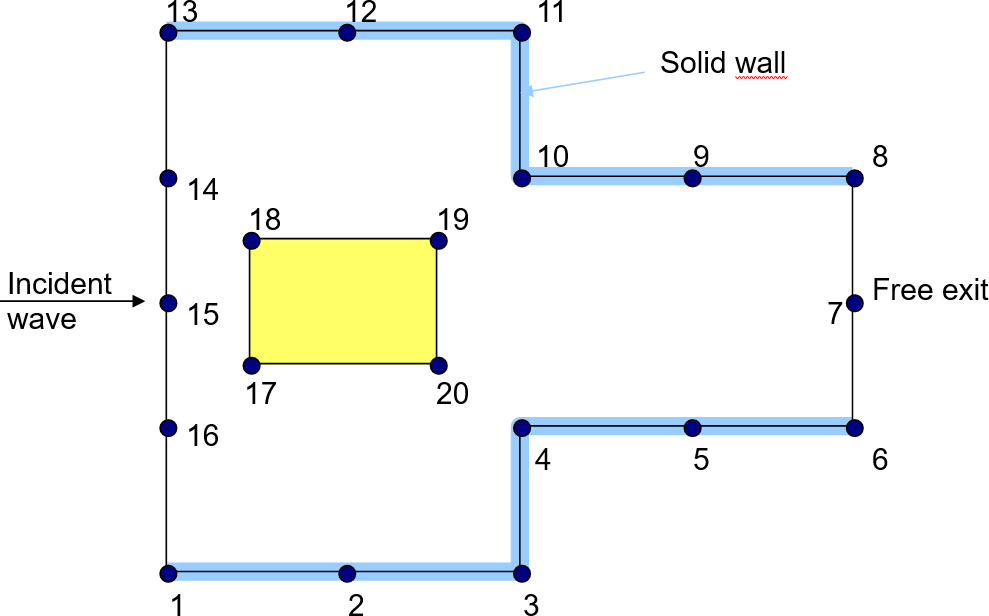
\includegraphics[width=\textwidth]{./graphics/bnd}
%
\caption{Schematic domain illustrating boundary condition coding}\label{fig:bnd}
\end{center}
\end{figure}

\begin{table}[H]
\begin{tabular}{|p{1.7in}|p{0.4in}|p{1.0in}|p{1.0in}|} \hline
\textbf{1${}^{st}$ column}\newline \textbf{Type of boundary condition} &  & \textbf{Penultimate column}\newline \textbf{General number} & \textbf{Last column}\newline \textbf{Boundary node number} \\ \hline
1 & \ldots & \ldots & 1 \\ \hline
2 & \ldots & \ldots & 2 \\ \hline
2 & \ldots & \ldots & 3 \\ \hline
2 & \ldots & \ldots & 4 \\ \hline
2 & \ldots & \ldots & 5 \\ \hline
4 & \ldots & \ldots & 6 \\ \hline
4 & \ldots & \ldots & 7 \\ \hline
4 & \ldots & \ldots & 8 \\ \hline
2 & \ldots & \ldots & 9 \\ \hline
2 & \ldots & \ldots & 10 \\ \hline
2 & \ldots & \ldots & 11 \\ \hline
2 & \ldots & \ldots & 12 \\ \hline
1 & \ldots & \ldots & 13 \\ \hline
1 & \ldots & \ldots & 14 \\ \hline
1 & \ldots & \ldots & 15 \\ \hline
1 & \ldots & \ldots & 16 \\ \hline
2 & \ldots & \ldots & 17 \\ \hline
2 & \ldots & \ldots & 18 \\ \hline
2 & \ldots & \ldots & 19 \\ \hline
\end{tabular}
  \caption{Example of boundary conditions file for the schematic case}\label{tab:bnd}
\end{table}


\section{Processing of solid boundaries (LIHBOR=KLOG)}

A solid boundary may reflect waves to varying degrees. It is therefore
necessary to characterise the wall reflection coefficient and also the possible
phase shift of the reflected waves in relation to the incident waves, produced
by the wall.

It must be stressed that in the case of a solid, the user must estimate
beforehand and as well as possible the angle of incident wave (or of main
incident wave constituent), even if this value is calculated by \artemis{}.

All the characteristics of the wall are determined in the subroutine BORH\@. The
values of the following parameters are specified for each solid boundary
(identified by the number of the boundary nodes):

\begin{itemize}
\item  RP : Reflection coefficient (between 0 and 1, with 1 corresponding to a
  perfectly reflecting wall, and 0 to a completely absorbing one)

\item  TETAP : Angle of incident wave attack in relation to the outward normal,
  expressed in degrees in the clockwise direction. It should be noted that the
    sign of this value is of no importance, since it only appears in the
    calculation in cosine form.

\item  ALFAP : Value of the phase shift produced by the wall (positive if the
  reflected wave is delayed in relation to the incident wave), expressed in
    degrees. If ALFAP=0, the coefficient RP corresponds exactly to the
    definition of the reflection coefficient, i.e.\ H${}_{totale}$ =
    H${}_{incidente}$ (1 + RP).
\end{itemize}

In the absence of any special programming in BORH, solid walls are all
considered as being perfectly reflecting and do not produce any phase shift
(RP=1, TETAP=ALFAP=0).

The following example shows a definition of two solid boundaries. The first is
a wall with pure reflection, and the second one that is partially reflecting,
generating a delay of 45$\mathrm{{}^\circ}$ when the incident wave has an angle
of 30$\mathrm{{}^\circ}$.

\begin{lstlisting}[language=Fortran]
      DO 10 I=1,20
         RP(I) = 1.D0
10    CONTINUE

      DO 20 I=32,40
         RP(I) = 0.5D0
         TETAP(I) = 30.D0
         ALPHAALFAP(I) = 45.D0
20    CONTINUE
\end{lstlisting}

The user may consult~\cite{Dhellemmes2003} for an estimate of the various
parameters.


\section{Processing of liquid}

Liquid boundaries can be of two types:

\begin{itemize}
\item  incident wave type

\item  incident potential type

\item  free exit type.
\end{itemize}


\subsection{Incident wave (LIHBOR=KINC)}

An incident wave type boundary allows waves arriving from offshore to enter and
waves from inside the domain to exit freely. From the theoretical standpoint,
the potential at such a boundary is a known potential (incident waves)
superimposed on an unknown potential (exiting waves).

In ARTEMIS, incident wave type boundaries enable waves arriving with an angle
TETAP to leave the domain (N.B. this should not be confused with the angle of
the incident waves TETAB).

From the point of view of the user, it is therefore necessary to provide the
characteristics of the incident wave and the value of the angle TETAP.

The characteristics of the incident wave are performed through the variables
HB, TETAB and TETAP in the BORH subroutine:

\begin{itemize}
\item HB: Wave height (monochromatic wave, see {\S} 7.1) or significant wave
  height (random wave, see {\S} 7.2)

\item TETAB: Propagation direction expressed in degrees in the trigonometric
  direction from the X-axis. This value can be imposed as space constant
  overall the domain through the keyword \textit{DIRECTION OF WAVE PROPAGATION}
  in the steering file.

\item ALFAP: Phase of the wave at the considered node, in degreessteering file.
  The user has to choose a reference point where the phase is zero. If the full
  boundary is perpendicular to the propagation direction, then ALFAP will be
  zero for the whole boundary nodes. A way to specify ALFAP can be found in
  some test cases (BTWI,CREOCEAN,ILE\_PARA) or in section 6.4.4.

\item TETAP: Output direction of waves reflected inside the domain (a priori
  unknown). TETAP defines the non-oriented angle between the forecast output
  direction of the wave and the boundary normal. This value is between 0 and
  $\pi$/2 and must be given in degres.
\end{itemize}

\subsection{Incident potential (LIHBOR=KPOT)}

An incident potential type boundary allows specifying a more general form of
the reduced potential, waves from inside the domain can still exit freely. From
the theoretical standpoint, the potential at such a boundary is a known
potential superimposed on an unknown potential (exiting waves). In ARTEMIS,
incident potential type boundaries enable waves arriving with an angle TETAP to
leave the domain.

From the point of view of the user, it is therefore necessary to provide the
characteristics of the incident wave and the value of the angle TETAP.

The characteristics of the incident potential are performed through the
variables (given in the BORH subroutine):

\begin{itemize}
  \item PRB:  Real part of the incident potential

  \item PIB: Imaginary part of the incident potential

  \item DDXPRB:  Real part of the derivative of incident
    potential with respect to X

  \item DDYPRB:  Real part of the derivative of incident
    potential with respect to Y

  \item DDXPIB:  Imaginary part of the derivative of incident
    potential with respect to X

  \item DDYPIB:  Imaginary part of the derivative of incident
    potential with respect to Y

  \item TETAP : Output direction of waves reflected inside the domain (a priori
    unknown). TETAP defines the non-oriented angle between the forecast output
    direction of the wave and the boundary normal. This value is between 0 and
    $\pi$/2 and must be given in degrees.

\end{itemize}

Note that this option has been validated in regular waves only. Considering the actual configuration of ARTEMIS, It should work in non-regular waves also, but no test has been performed yet.


\subsection{Free exit (LIHBOR=KSORT)}

This type of boundary allows waves to leave freely. However, this type of exit
is only free in ARTEMIS in the case of waves attacking the boundary at an angle
TETAP\@. It is therefore necessary for the user to estimate the angle of attack
of exiting waves beforehand.

TETAP is programmed in the subroutine BORH\@. The default value (TETAP=0) enables
waves normal to the boundary to exit.

\subsection{Modifications of «~incident wave~» boundary condition from V6P2}

From version V6P2 of ARTEMIS, the user needs to define the phase of the incident wave by himself. This operation was done automatically by the code until V6P1. The reasons for changing are the following:

\begin{itemize}
\item  From a physical point of view, the automatic phase calculation is not satisfying. In particular when the wave number and the water depth are variable in space.

\item  From a computing point of view, the automatic calculation in not really compatible with parallel computation.
\end{itemize}

Thus, the user has to give the phase in the ALFAP table, for each point of «~incident wave» type (LIHBOR\%I=KINC). Users will find bellow some examples of how to calculate the phase.

\underbar{Example 1}: incident wave normal to the boundary

    \begin{minipage}[b]{0.5\textwidth}
In that case, the phase can be set to 0 on the whole boundary.

    \end{minipage}%
    \begin{minipage}[b]{0.4\textwidth}
      \begin{figure}[H]%
        \centering
        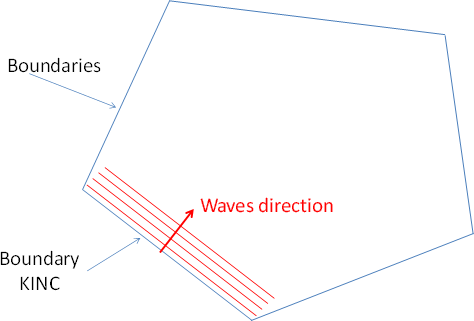
\includegraphics[width=\textwidth]{./graphics/example1}
      \end{figure}
    \end{minipage}%

\underbar{Example 2}: incident wave not normal to the boundary, constant bathymetry

    \begin{minipage}[b]{0.6\textwidth}
      In that case, the phase at point I can be calculated using the following
      formula~(users need to choose a reference point A):\\
      $\varphi_{I} =k\cdot \cos \theta \cdot (x_{I} -x_{A} )+
        k\cdot \sin \theta \cdot (y_{I} -y_{A})$

    \end{minipage}%
    \begin{minipage}[b]{0.4\textwidth}
      \begin{figure}[H]%
        \centering
        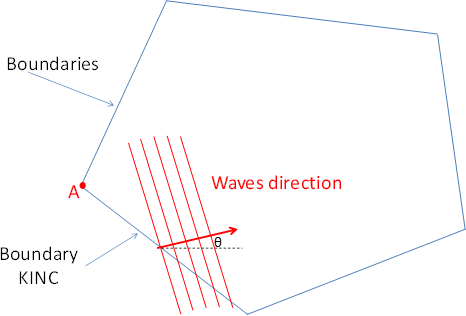
\includegraphics[width=\textwidth]{./graphics/example2}
      \end{figure}
    \end{minipage}%


\underbar{Example 3}: incident wave not normal to the boundary, variable bathymetry

The automatic calculation done by Artemis until version V6P1 used an
incremental formulation on the boundary~(see test cases BTWI or CREOCEAN) from
a given point A:
\[\varphi _{I} =\sum _{P=A}^{I-1}k(P)\cdot \cos \theta \cdot \left(x_{P+1} -x_{P} \right) +k(P)\cdot \sin \theta \cdot \left(y_{P+1} -y_{P} \right)\]
Another option is to choose a characteristic water depth of the boundary, then
to calculate a characteristic wave number k${}_{ref}$ and to use the formula
(see parallel version of test BTWI):
\[\varphi _{I} =k_{ref} \cdot \cos \theta \cdot (x_{I} -x_{A} )+k_{ref} \cdot \sin \theta \cdot (y_{I} -y_{A} )\]


\underbar{Example 4}: Variation in wave direction.

This case is not really recommended, or should at least need a specific
attention. The best option is probably to perform several computations with
random phases and to consider mean values.



As a conclusion, it is recommended to define an ``incident wave'' boundary as
representative as possible of a far field wave field, so to respect the
following recommendations for each boundary:

\begin{itemize}
\item  Reasonable topography variations on the boundary.

\item  No variation in the waves direction

\item  Incident wave condition applied near a solid boundary in the interest area, or in a corner, can generate local effects on the results. The interest area has to be far from those local effects.
\end{itemize}

\eject


\chapter{Physical parameters}

Physical parameters are introduced essentially to characterise the type of
calculation that is to be performed (regular waves, random waves, period
scanning) and the dissipation phenomena taken into account (breaking, bottom
friction).

The detailed list of keywords used by \artemis{}, and classified by
alphabetical order, is supplied in Appendix 4.


\section{Monochromatic waves}

The simplest type of calculation of course concerns monochromatic
wavesmonochromatic waves. In this case, the user supplies the height of
the incident waves in metres (HB) and their direction identified by the angle
TETAB (in degrees) made between the incident wave vector and the X-axis
(reckoned positively in a clockwise direction). This definition must be entered
in the subroutine BORH\@. The wave period, expressed in seconds, is
supplied with the key word \textit{WAVE PERIOD}.

If the user only wishes to specify a single incident wave direction (or when
there is only one incident wave boundary), the data can be supplied more easily
with the key word \textit{DIRECTION OF WAVE PROPAGATION} In this case, this
value is assigned to all the boundaries concerned. It should also be noted that
the wave height is fixed by default at 1m for all boundaries.

In the case of several boundaries with different incident wave directions, it
is necessary to use the subroutine BORH.


\section{Random waves}

In reality, waves are random. This can be interpreted as the superimposition of
several monochromatic waves of different periods that are randomly out of phase
with one another. In this case, the real wave energy is the sum of the energies
of the component monochromatic waves. The curve showing energy density as a
function of frequency is referred to as the ``energy spectrum'' (see {\S} 3.6).

Numerically speaking, the principle adopted in \artemis{} involves discretizing
the energy spectrum into a number of bands of equal energy in order to perform
a calculation in regular wave conditions for each of the characteristic
frequencies of each band. ARTEMIS then recombines the various results in order
to determine the overall wave height.

In the case of multi-directional waves, the principle is the same. The
direction spectrum is broken down into bands of equal energy.

The random character of the waves is taken into account by activating the key
words \textit{MONODIRECTIONAL RANDOM WAVE} and \textit{MULTIDIRECTIONAL RANDOM
WAVE}, as the case may be.

In order to discretize the energy spectrum, it is necessary on the one hand to
fix the energy spectrum peak period (given by the key word \textit{PEAK
PERIOD}, and the number of bands of equal energy that the user
wishes to use (given by the key word \textit{NUMBER OF
PERIODS}, which has a default value of 5). Moreover, the two key words
\textit{MINIMUM SPECTRAL PERIOD} (default value 0.02)
and \textit{MAXIMUM SPECTRAL PERIOD} (default value 200)
are used to specify the limits of the spectrum. The key word
\textit{GAMMA} is used to specify the value of the coefficient $\gamma$
involved in Goda's formula (cf. {\S} 3.6). This key word can have values of
between 1 and 7. The value 1 corresponds to a spectrum of the
Pierson-Moskowitz type, and 3.3 (default value) to a mean Jonswap spectrum.

In the case of a multi-directional waves, the user must provide the boundaries
of the direction spectrum (using the key words \textit{MINIMUM ANGLE OF
PROPAGATION} and \textit{MAXIMUM ANGLE OF PROPAGATION} ), together with the
number of bands using the key word \textit{NUMBER OF DIRECTIONS} (default value
5). The maximum value of the exponent s involved in the expression giving the
directional distribution of the wave energy (cf. {\S} 3.6) is specified with
the key word \textit{S EXPONENT} (default value 20).


\section{Period scanning. Resonance}

ARTEMIS offers the possibility of performing a calculation in monochromatic
wave conditions by varying the wave period over a range of values defined by
the user. This technique is used more particularly when searching for resonance
frequencies (for example when introducing a wave into a closed basin).

This option is activated with the logical key word \textit{PERIOD SCANNING}.
The user must also provide the boundaries of the scanning range using the real
key words \textit{BEGINNING PERIOD FOR PERIOD SCANNING} and \textit{ENDING
PERIOD FOR PERIOD SCANNING}. The scanning step is specified with the key word
\textit{STEP FOR PERIOD SCANNING}. All these values are fixed at zero by
default.

In this case, ARTEMIS performs a calculation for each of the periods specified.
The results are stored in the results file (with period sampling if the key
word \textit{GRAPHIC PRINTOUT PERIOD}word \textit{GRAPHIC PRINTOUT PERIOD} is
used).


\section{Bathymetric breaking}

ARTEMIS offers the possibility of including dissipation due to bathymetric wave
breaking, for example when the waves reach a beach (bathymetric breaking is
used in opposition to offshore white-capping.

ARTEMIS offers two formulations for regular wave breaking: that of Battjes and
Janssen, and that of Dally. Only the first is available for random waves.

This phenomenon is taken into account by activating the logical key word
\textit{BREAKING} (default value NO). The formulation to be used (cf. {\S}
3.4.1) is then specified with the key word \textit{BREAKING LAW}, which may
have the value 1 (Battjes and Janssen) or 2 (Dally) (default value 1). Lastly,
the value of the coefficient $\gamma_{s}$ in the breaking height criterion (cf.
{\S} 3.4.1.1) is given with the key word \textit{GAMMAS} (default value 0.88),
which is not to be confused with the key word \textit{GAMMA} in the energy
spectrum formula (cf. {\S} 3.6).

In the case of Dally's formula, the coefficients $\Gamma$ and K are provided
with the key words \textit{GDALLY} (default value 0.4) and \textit{KDALLY}
(default value 0.1). In the case of Battjes and Janssen's formula, the
coefficient $\alpha$ is provided with the key word\textit{ALPHA} (cf. {\S}
3.4.1.2).

In a calculation that takes into account breaking, the mnemonic QB is added in
the list of the key word \textit{VARIABLES FOR GRAPHIC PRINTOUTS} in order to
obtain the rate of breaking calculated by the software. This rate, which is
between 0 and 1, represents the percentage of waves that break in the case of a
random wave simulation. With monochromatic wave simulations, the breaking rate
is 1 or 0.


\section{Bottom friction}

ARTEMIS allows dissipation due to bottom friction to be
taken into account. This is done by using the formulation of Kostense et al.\ or
that of Putnam and Johnson.

Bottom friction is a complex question involving many notions that are described
in {\S} 3.4.2.

The key word \textit{FRICTION} (default value NO) is used to take this into
account in the calculation.


\subsection{Determination of friction factor}

The friction factor is either supplied by the user or determined directly by
ARTEMIS in the case of a \textbf{sandy} bed.

In order to introduce the friction factor directly, it is necessary to activate
the logical key word \textit{FRICTION FACTOR IMPOSED}. If this is spatially
constant, the value may be specified simply by using the key word
\textit{FRICTION FACTOR} (default value 0). If not, it is necessary to enter
the subroutine FWSPEC, and assign a friction factor value to the variable FW at
each mesh node (to do this, it is possible to use the subroutine FILPOL, which
enables the value of any variable to be prescribed inside a polygon).

If the keyword \textit{FRICTION FACTOR IMPOSED} = FALSE (default value),
ARTEMIS assumes that the bed is sandy. In this case, the friction factor
determination formulae built into ARTEMIS are used. The main consideration is
the hydraulic regime. Here again, the regime may be determined automatically by
ARTEMIS at each mesh point, or specified directly by the user. The latter
option is activated using the logic key word \textit{HYDRAULIC REGIME IMPOSED}
(default value NO), and the type of regime is then given by the key word
\textit{HYDRAULIC REGIME TYPE}, which may have any of the following values:

\begin{itemize}
\item  1 : laminar regime

\item  2 : smooth turbulent regime

\item  3 : rough turbulent regime

\item  4 : transient regime
\end{itemize}

Depending on the hydraulic regime, the friction factor is calculated by means
of various formulae, in which the various parameters must be supplied using key
words (see {\S} 3.4.2).

In the case of a rough turbulent regime, the friction factor depends on the
skin roughness, which is connected with the size of the sediment particles, and
on the shape roughness, which is connected with the appearance of undulations
on the ground referred to as ripples. ARTEMIS enables the user to ignore shape
roughness by activating the logic key word \textit{SKIN ROUGHNESS ONLY}
(default value NO). In this case, the roughness value is taken to be equal to
three times the value supplied by the key word \textit{DIAMETER90} described
below.

The other key words used to supply the physical parameters needed for ARTEMIS
to take into account friction on a sandy bed are the following:

\begin{itemize}
\item  The key word \textit{FLUID KINEMATIC VISCOSITY} (default value
  10${}^{-6}$ m${}^{2}$/s) provides the viscosity of the water.

\item  Key words \textit{FLUID SPECIFIC MASS }(default value 1000 kg/m${}^{3}$)
  and \textit{SEDIMENT SPECIFIC WEIGHT }(default value 2650 kg/m${}^{3}$) are
    used to supply the water and sand densities for rough turbulent or
    transient hydraulic regimes.
\end{itemize}

The size of the sediment particles involved in determining the bottom friction
factor is indicated with the following key words:

\begin{itemize}
\item  Key word \textit{DIAMETER50} (default value 0.1x10${}^{-3}$) indicates
  the maximum size of 50\% of the volume of sediment. The values generally used
    are:

\begin{itemize}
\item  0.66x10${}^{-3}$ for very coarse sand,

\item  0.33x10${}^{-3\ }$for coarse sand,

\item  0.17x10${}^{-3}$ for medium sand,

\item  0.083x10${}^{-3}$ for fine sand,

\item  0.04x10${}^{-3}$ for very fine sand.
\end{itemize}

\item  Key word \textit{DIAMETER90} (default value 0.15x10${}^{-3}$) indicates
  the maximum size of 90\% of the volume of sediment. The values generally used
    are:

\begin{itemize}
\item  10${}^{-3}$ for very coarse sand,

\item  0.5x10${}^{-3}$ for coarse sand,

\item  0.25x10${}^{-3}$ for medium sand,

\item  0.125x10${}^{-3}$ for fine sand,

\item  0.062x10${}^{-3}$ for very fine sand.
\end{itemize}

\item  Key word \textit{RIPPLES COEFFICIENT} (default value 0.7) indicates the
  value of the ripple coefficient when shape roughness is taken into account.
    This key word can have the following values:

\begin{itemize}
\item  1 for ripples only,

\item  0.7 when the ripples are superimposed on sand waves.
\end{itemize}
\end{itemize}


\subsection{Determination of dissipation coefficient}

Once the friction factor has been determined, it is possible to calculate the
value of the dissipation term associated with the bottom friction.

ARTEMIS can calculate the dissipation term by one of two different formulae,
that of Kostense, Meijer and Dingemans, or that of Putnam and Johnson.

The formula is chosen (cf. {\S} 3.4.2) with the key word \textit{BOTTOM
FRICTION LAW}, which can have the following values:

\begin{itemize}
\item  1 for Kostense et al.'s formula (default value)

\item  2 for Putnam and Johnson's formula.
\end{itemize}


\section{Rapidly varying topography}

Since version 6.1, user can take into account second order bottom effects. To
use this option, the keyword «~RAPIDLY VARYING TOPOGRAPHY~» must appear in the
case file.

The equation solved and the model choice is given in 1.3.1.3. The reader can
find in 1.4.1 des informations d\'{e}taill\'{e}es sur l'impl\'{e}mentation et
l'utilisation de cette option.

The keyword «~RAPIDLY VARYING TOPOGRAPHY~» can take the values 0,1,2 or 3.
\begin{itemize}
  \item 0: correspond to classical mild-slope equation.
  \item 1: gradient effects are taken into account.
  \item 2: curvature effects are taken into account.
  \item 3: both gradient
and curvature effects are taken into account.
\end{itemize}

Defaut value: 0.

\section{Other parameters}

The key word \textit{GRAVITY ACCELERATION} (default value 9.81) is used to
specify the acceleration due to gravity in m/s${}^{2}$.


\chapter{General parameters}

The general parameters for the calculation are indicated only in the parameters
file (see Appendix 4).

The title of the calculation is specified with the key word \textit{TITLE}.

If a vector computer is being used, it is necessary to specify the vector
length with the key word \textit{VECTOR LENGTH}. The default value of this key
word (1) corresponds to a scalar computer (i.e.\ the case with
workstations).

When generating an executable, the libraries used to edit the links and the
version of the libraries are specified with the key words \textit{LIBRARIES}
and \textit{RELEASE}. When the software is installed on a workstation, the
default value of these key words is often sufficient.


\chapter{Numerical parameters}

A number of key words enable the user to configure an ARTEMIS calculation from
the numerical standpoint (see Appendix 4).


\section{Solver}

Firstly, the integer key word \textit{SOLVER} is used to choose the solver for
the system of equations processed by \artemis{}. The possible values are:

\begin{itemize}
  \item 1: Conjugated gradient,
  \item 2: Conjugated residual,
  \item 3: Conjugated gradient on normal equation,
  \item 4: Minimum error,
  \item 6: Conjugated gradient of CGSTAB type,
  \item 7: GMRES
  \item 8: Direct solver
\end{itemize}

By default, ARTEMIS uses the direct solver (option 8).

When option 7 is used, the size of the Krylov space is specified with the key word \textit{SOLVER OPTION}.

It should be stressed that:

\begin{itemize}
\item  in the present state of development of ARTEMIS, the solver GMRES (option
  7) does not appear to give satisfactory results;

\item  The number of iteration require by the iterative solver to obtain a
  solution for the linear system is often high. By consequence, using such
    method is less interesting than a formal matrix inversion like with the
    direct solver;

\item  When you use the direct solver for large mesh sizes, you may need to
  increase the parameter MEMFACTOR in the new subroutine SD\_SOLVE\_1.f.
\end{itemize}


\section{Accuracy}

When the linear system is solved by an iterative method. It is therefore
necessary to define the accuracy that one wishes to obtain during the
calculation, and the maximum permissible number of iterations, so as to avoid
looping if the required level of precision is not attained.

The level of accuracy is specified with the key word \textit{SOLVER ACCURACY}
(default value 10${}^{-4}$). The maximum number of iterations is specified with
the key word \textit{MAXIMUM NUMBER OF ITERATIONS FOR SOLVER} (default value
60000).

The user may obtain information on the solver by activating the key word
\textit{INFORMATION ABOUT SOLVERINFORMATION ABOUT SOLVER} (default value YES).
This information is supplied in the printout, and may be of two types:

\begin{itemize}
\item  Either the process has converged before reaching the maximum permitted
  number of iterations, and in this case ARTEMIS indicates the number of
    iterations actually run, together with the precision attained.

\item  Or the process has not converged sufficiently quickly, the ARTEMIS then
  displays the message ``MAXIMUM NUMBER OF ITERATIONS REACHED'' and indicates
    the precision actually attained.
\end{itemize}


\section{Preconditioning}

When the system of equations is solved by a conjugated gradient method,
convergence may often be speeded up by preconditioning.

ARTEMIS offers several preconditioning options. The key word
\textit{PRECONDITIONING} is used to choose the type required:

\begin{itemize}
\item  0 : no preconditioning,

\item  2 : diagonal preconditioning (default value),

\item  3 : diagonal preconditioning with condensed matrix,

\item  5 : diagonal preconditioning in absolute values,

\item  7 : Crout's preconditioning per element.
\end{itemize}

Certain types of preconditioning can be cumulated, such as the diagonals with
the others. The basic values are prime numbers, so that two types of
preconditioning can be cumulated by assigning to the key word the product of
the corresponding two prime numbers, e.g. 6 corresponds to types 2 and 3.


\section{Handling of cases with energy dissipation}

When the calculation has to take into account dissipation phenomena (breaking,
bottom friction or both), \artemis{} first of all runs a calculation without
taking the dissipation into account. This first solution is then used to
determine an initial value of the dissipation term to be introduced into the
mild slope equation. ARTEMIS then runs a second calculation, taking into
account the new term. The process is then iterated until a satisfactory
solution is obtained. As with the precision of the general solver (see {\S}
9.2), the user may configure the convergence criteria of these iterations by
using the key word \textit{SUB-ITERATIONS ACCURACY} (default value 10-2) and
the maximum number of iterations using the key word \textit{MAXIMUM
SUB-ITERATIONS} (default value 15).

As with the general solver, ARTEMIS provides information concerning this
process in the control printout if the key word \textit{INFORMATION ABOUT
SOLVER} is activated (default value YES). In particular, \artemis{} provides
the maximum difference between each sub-iteration and the previous one
(expressed as a percentage).

Lastly, a relaxation coefficient is introduced at each iteration, when the
dissipation coefficient is calculated, in order to avoid oscillations in solver
convergence. This coefficient is specified by means of the key word
\textit{DISSIPATION RELAXATION} (default value 0.5). It is introduced in the
form:

MU2 = MU1 + RELAX*(MU2-MU1)

where
\begin{itemize}
  \item MU2 is the dissipation term calculated during the current iteration,
  \item MU1 is the dissipation term calculated during the previous iteration,
  \item RELAX is the relaxation coefficient.
\end{itemize}

The user may need to reduce the value of the relaxation coefficient,
particularly in the case of regular waves.


\chapter{Programming of complex cases}


\section{Modification of bed elevation (corfon)}

The sea bottom may be introduced at various levels, as indicated in {\S} 4.4.

ARTEMIS offers the possibility of modifying the bottom at the start of the
calculation, using the subroutine CORFON\@. This subroutine is used to modify the
value of the variable ZF at each mesh point. To do so, the user can change a
number of variables, such as, for example, the point coordinates (X and Y), the
area of the elements, the table of connectivities, etc.

By default, the subroutine CORFON performs LISFON bottom smoothing, i.e.\ as
many as are specified by the key word \textit{BOTTOM TOPOGRAPHY SMOOTHING}
(default value 0).


\section{Modification of coordinates (corrxy)}

ARTEMIS also offers the possibility of modifying the coordinates of the mesh
points. In this way it is possible to change, for example, the scale
(transition from a scale model to real size), make a rotation or lateral
displacement, etc.

This is done by using the subroutine CORRXY, which is called up at the start of
the calculation. By default, this subroutine is empty and shows an example of
programming concerning a change of scale and origin, in the form of comment
lines.


\section{Addition of new variables}

ARTEMIS allows the user to create new variables. The names of these new
variables must be declared in the subroutine NOMVAR in the form of a mnemonic
of no more than 8 characters.

Secondly, the user must calculate the value of these new variables in the
subroutine UTIMP\@. To do this, he can use the tables PRIVE (dimension (number of
points, NPRIV)) to transmit information between the various user-accessible
subroutines. When these tables are being used, it is necessary to give their
number (NPRIV value) in the main program.


\chapter{Other}

\section{Running an ARTEMIS computation}

computation is started using the command \artemis{}. This command activates the
execution of a unix script which is common to all the computation modules of
the TELEMAC modelling system.

The syntaxes of this command are as follows:

artemis [options] [cas]

Les options possibles sont:

\begin{itemize}
\item  -s: When using in interactiv mode, generates a copy of the output listing on disk (by default, the output listing is only displayed on screen)

\item  -D: Compilation and execution using a debugger.

\item  -t: The temporarily directory is not erased at the end of the computation

\item  -cl: Compilation and link without execution.

\item  -noautopar: parallel computation not enable (no partitioning of the model)

\item  -b: Compilation and execution in batch mode (immediate start).

\item  -n: Compilation and execution in deferred batch mode (start at 20h00).

\item  -d: Compilation and execution in deferred batch mode (start at the specified time).

\item  Cas: Name of steering file.
\end{itemize}

\artemis{} --h {\textbar} -H  (short or long help).

If no name for the steering file is indicated, the procedure uses
the name `cas'. By default, the procedure executes the computation in
interactive mode.

The following operations are carried out using this script:

\begin{itemize}
\item  Creation of a temporary directory,

\item  Copy of the dictionary and steering file in this directory,

\item  Execution of DAMOCLES software in order to determine the name of the work files,

\item  Creation of the script to start the computation,

\item  Allocation of files,

\item  Compilation of the FORTRANFORTRAN file and link edition (if necessary)

\item  Start of the computation,

\item  Restitution of the results files, and erasing of the temporary directory.
\end{itemize}

Procedure operation differs slightly depending on the options used.

A detailed description of this procedure may be obtained by using the command \artemis{} -H.

\eject

\section{List of subroutines most frequently modified by users}

\begin{itemize}
\item BORH Prescription of boundary conditions

\item BORH\_EX\_COUPLING\_TOMAWAC Exemple of prescription of boundary conditions comming from a TOMAWAC result

\item CONDIH Definition of initial conditions

\item CORFON Modification of topography

\item FWSPEC Space varying friction coefficient

\item NOMVAR\_ARTEMIS Definition of names of additional user variables

\item SD\_SOLVE1 Direct solver (to modify the MEMFACTOR parameter if it should be increase)

\item UTIMP Additional programming
\end{itemize}

\section{Example of a steering file}
\begin{lstlisting}[language=TelemacCas]
/-------------------------------------------------------------------
/ ARTEMIS Version v6p2 juillet 2012
/ VALIDATION ARTEMIS - TEST Battjes \& Janssen 1978, RUN 15
/-------------------------------------------------------------------
/-------------------------------------------------------------------
/ INITIAL CONDITIONS EQUATIONS
/-------------------------------------------------------------------
INITIAL CONDITIONS ='CONSTANT ELEVATION'
INITIAL WATER LEVEL =0.
/-------------------------------------------------------------------
/ INPUT-OUTPUT,FILES
/-------------------------------------------------------------------
FORTRAN FILE ='art\_bj78-princi.f'
RESULTS FILE ='art\_bj78-scal.res'
REFERENCE FILE ='ref\_bj78.res'
BOUNDARY CONDITIONS FILE ='geo\_bj78.cli'
GEOMETRY FILE ='geo\_bj78.slf'
/-------------------------------------------------------------------
/ INPUT-OUTPUT,GRAPHICS AND LISTING
/-------------------------------------------------------------------
VARIABLES FOR GRAPHIC PRINTOUTS=
'HS,ZF,QB,SXX,SXY,SYY,FX,FY,T01,T02,TM,INC,K,C,CG'
VALIDATION =YES
/-------------------------------------------------------------------
/ INPUT-OUTPUT,INFORMATION
/-------------------------------------------------------------------
TITLE ='VALIDATION ARTEMIS 6.0 - TEST Battjes \& Janssen 1978, RUN 15'
/-------------------------------------------------------------------
/ NUMERICAL PARAMETERS
/-------------------------------------------------------------------
NUMBER OF PRIVATE VARIABLES =4
SOLVER = 8
/for parallel calculations using n processors
/add PARALLEL PROCESSORS : n
/replace SOLVER : 8 by SOLVER : 3
/-------------------------------------------------------------------
/ PHYSICAL PARAMETERS
/-------------------------------------------------------------------
BREAKING =YES
DIRECTION OF WAVE PROPAGATION =0.
MAXIMUM SPECTRAL PERIOD =8.
PEAK PERIOD =1.887
MONODIRECTIONAL RANDOM WAVE =YES
MINIMUM SPECTRAL PERIOD =0.75
GAMMA =3.3
\end{lstlisting}

\section{Example of a user Fortran Fortran file}
\begin{lstlisting}[language=TelFortran]
C                       ***************
                        SUBROUTINE BORH
C                       ***************
C
C***********************************************************************
C
C  ARTEMIS  VERSION 6.2 07/12
C  LINKED TO BIEF VERS. 6.2        J-M HERVOUET (LNH) 01 30 87 80 18
C
C***********************************************************************
C
C      FONCTION:    PREND EN COMPTE LES CONDITIONS AUX LIMITES
C                   DE L'UTILISATEUR
C                   ELLES SONT DONNEES PAR SEGMENT.
C
C      CE SOUS-PROGRAMME PEUT ETRE COMPLETE PAR L'UTILISATEUR
C
C-----------------------------------------------------------------------
C                             ARGUMENTS
C .________________.____.______________________________________________.
C |      NOM       |MODE|                   ROLE                       |
C |________________|____|______________________________________________|
C |   RP           |<-- |  COEFFICIENTS DE REFLEXION DES PAROIS        |
C |   TETAP        |<-- |  ANGLE D'ATTAQUE DE LA HOULE SUR LES LIMITES |
C |                |    |  PAS SEULEMENT LES PAROIS, MAIS AUSSI LES    |
C |                |    |  LES FRONTIERES LIQUIDES                     |
C |                |    |  (COMPTE PAR RAPPORT A LA NORMALE EXTERIEURE |
C |                |    |   DANS LE SENS DIRECT)                       |
C |   ALFAP        |<-- |  DEPHASAGE INDUIT PAR LA PAROI ENTRE L'ONDE  |
C |                |    |  REFLECHIE ET L'ONDE INCIDENTE (SI ALFAP EST |
C |                |    |  POSITIF, L'ONDE REFLECHIE EST EN RETARD)    |
C |   HB           |<-- |  HAUTEUR DE LA HOULE AUX FRONTIERES OUVERTES |
C |   TETAB        |<-- |  ANGLE D'ATTAQUE DE LA HOULE (FRONT. OUV.)   |
C |                |    |  (COMPTE PAR RAPPORT A L'AXE DES X DANS LE   |
C |                |    |   SENS DIRECT)                               |
C |    H           | -->|  HAUTEUR D'EAU                               |
C |    K           | -->|  NOMBRE D'ONDE                               |
C |    C,CG        | -->|  VITESSES DE PHASE ET DE GROUPE              |
C |    C           | -->|  CELERITE AU TEMPS N                         |
C |    ZF          | -->|  FOND                                        |
C |    X,Y         | -->|  COORDONNEES DES POINTS DU MAILLAGE          |
C |  TRA01,...,3   |<-->|  TABLEAUX DE TRAVAIL                         |
C | XSGBOR,YSGBOR  | -->|  NORMALES EXTERIEURES AUX SEGMENTS DE BORD   |
C |   LIHBOR       | -->|  CONDITIONS AUX LIMITES SUR H                |
C |    NBOR        | -->|  ADRESSES DES POINTS DE BORD                 |
C |   KP1BOR       | -->|  NUMERO DU POINT FRONTIERE SUIVANT           |
C |   OMEGA        | -->|  PULSATION DE LA HOULE                       |
C |   PER          | -->|  PERIODE DE LA HOULE                         |
C |   TETAH        | -->|  ANGLE DE PROPAGATION DE LA HOULE            |
C |   GRAV         | -->|  GRAVITE                                     |
C |   NPOIN        | -->|  NOMBRE DE POINTS DU MAILLAGE.               |
C |   NPTFR        | -->|  NOMBRE DE POINTS FRONTIERE.                 |
C |   KENT,KLOG    | -->|  CONVENTION POUR LES TYPES DE CONDITIONS AUX |
C |   KSORT,KINC   |    |  LIMITES                                     |
C |                |    |  KENT  : ENTREE (VALEUR IMPOSEE)             |
C |                |    |  KLOG  : PAROI                               |
C |                |    |  KSORT : SORTIE                              |
C |                |    |  KINC  : ONDE INCIDENTE                      |
C |   PRIVE        | -->|  TABLEAU DE TRAVAIL (DIMENSION DANS PRINCI)  |
C |________________|____|______________________________________________|
C MODE : -->(DONNEE NON MODIFIEE), <--(RESULTAT), <-->(DONNEE MODIFIEE)
C
C-----------------------------------------------------------------------
C
C APPELE PAR : ARTEMI
C
C***********************************************************************
C
      USE BIEF
      USE DECLARATIONS_TELEMAC
      USE DECLARATIONS_ARTEMIS
C
      IMPLICIT NONE
      INTEGER LNG,LU
      COMMON/INFO/LNG,LU
C
      INTEGER I,JB
C
      DOUBLE PRECISION PI,BID
      PARAMETER( PI = 3.1415926535897932384626433D0)
C
      INTRINSIC COS,SIN
C
C-----------------------------------------------------------------------
C
C CONDITIONS AUX LIMITES
C UN SEGMENT EST SOLIDE SI IL EST DE TYPE KLOG.
C UN SEGMENT EST ONDE INCIDENTE SI IL EST DE TYPE KINC.
C UN SEGMENT EST UNE ENTREE SI IL EST DE TYPE KENT.
C UN SEGMENT EST UNE SORTIE SI IL EST DE TYPE KSORT.
C
C TOUS LES ANGLES SONT EN DEGRES
C                         ------
C ---------------------------------------
C INITIALISATION DES VARIABLES PAR DEFAUT
C ---------------------------------------
      TETAB\%R(:) = TETAH
      TETAP\%R(:) = 0.D0
      ALFAP\%R(:) = 0.D0
      RP\%R(:)    = 0.D0
      HB\%R(:)    = 1.D0
C

      DO I=1,NPTFR
       JB=BOUNDARY_COLOUR\%I(I)
C -----------------------------
C EXEMPLE DE CONDITIONS LIMITES  :
C
C
C PAROIS SOLIDES
      IF(JB.GE.2.AND.JB.LE.139)THEN
         LIHBOR\%I(I) = KLOG
         RP\%R(I) = 1.D0
         TETAP\%R(I) = 90.D0
         ALFAP\%R(I) = 0.D0
      ENDIF
      IF(JB.GE.146.AND.JB.LE.283)THEN
         LIHBOR\%I(I) = KLOG
         RP\%R(I) = 1.D0
         TETAP\%R(I) = 90.D0
         ALFAP\%R(I) = 0.D0
      ENDIF
C
C
C PAROIS AUX FRONTIERES OUVERTES
C
      IF(JB.GE.140.AND.JB.LE.145)THEN
         LIHBOR\%I(I) = KSORT
         TETAP\%R(I) = 0.D0
      ENDIF
C
C
C FRONTIERE ONDE INCIDENTE
C
      IF(JB.GE.284.AND.JB.LE.288)THEN
       LIHBOR\%I(I) = KINC
       HB\%R(I) = 0.202D0
       TETAB\%R(I) = 0.D0
       TETAP\%R(I) = 0.D0
       ALFAP\%R(I) = 0.D0
      ENDIF

      IF(JB.EQ.1)THEN
       LIHBOR\%I(I) = KINC
       HB\%R(I) = 0.202D0
       TETAB\%R(I) = 0.D0
       TETAP\%R(I) = 0.D0
       ALFAP\%R(I) = 0.D0
      ENDIF

      ENDDO
C
C POUR UN CALCUL EN HOULE ALEATOIRE MULTIDIRECTIONNELLE, LE CODE
C CALCULE LES DIRECTIONS DE PROPAGATION A PARTIR DES DONNEES DU FICHIER
C DES MOTS CLES.
C
C
C-----------------------------------------------------------------------
C
C
      RETURN
      END
C                       *****************
                        SUBROUTINE CORFON
C                       *****************
C
C***********************************************************************
C PROGICIEL : TELEMAC 5.0          01/03/90    J-M HERVOUET
C***********************************************************************
C
C  USER SUBROUTINE CORFON
C
C  FUNCTION  : MODIFICATION OF THE BOTTOM TOPOGRAPHY
C
C
C-----------------------------------------------------------------------
C .________________.____.______________________________________________
C |      NOM       |MODE|                   ROLE
C |________________|____|_______________________________________________
C |      ZF        |<-->| FOND A MODIFIER.
C |      X,Y,(Z)   | -->| COORDONNEES DU MAILLAGE (Z N'EST PAS EMPLOYE).
C |      A         |<-- | MATRICE
C |      T1,2      | -->| TABLEAUX DE TRAVAIL (DIMENSION NPOIN)
C |      W1        | -->| TABLEAU DE TRAVAIL (DIMENSION 3 * NELEM)
C |      NPOIN     | -->| NOMBRE DE POINTS DU MAILLAGE.
C |      PRIVE     | -->| TABLEAU PRIVE POUR L'UTILISATEUR.
C |      LISFON    | -->| NOMBRE DE LISSAGES DU FOND.
C |________________|____|______________________________________________
C MODE : -->(DONNEE NON MODIFIEE), <--(RESULTAT), <-->(DONNEE MODIFIEE)
C-----------------------------------------------------------------------
C
C PROGRAMME APPELANT :
C PROGRAMMES APPELES : RIEN EN STANDARD
C
C***********************************************************************
C
      USE BIEF
      USE DECLARATIONS_ARTEMIS
C
      IMPLICIT NONE
      INTEGER LNG,LU
      COMMON/INFO/LNG,LU
C
      INTEGER I
C
C+-+-+-+-+-+-+-+-+-+-+-+-+-+-+-+-+-+-+-+-+-+-+-+-+-+-+-+-+-+-+-+-+-+-+-+
C
C
C+-+-+-+-+-+-+-+-+-+-+-+-+-+-+-+-+-+-+-+-+-+-+-+-+-+-+-+-+-+-+-+-+-+-+-+
C
      LOGICAL MAS
C
C-----------------------------------------------------------------------
C
C  LISSAGES EVENTUELS DU FOND
C
      IF(LISFON.GT.0) THEN
C
        MAS=.TRUE.
        CALL FILTER(ZF,MAS,T1,T2,AM1,'MATMAS          ',
     *              1.D0,T1,T1,T1,T1,T1,T1,MESH,MSK,MASKEL,LISFON)
C
      ENDIF
C
C-----------------------------------------------------------------------
C
      DO 20 I = 1,NPOIN
         IF (X(I).LT.-5.D0) THEN
            ZF\%R(I) = -0.616D0
         ENDIF
         IF (X(I).GE.-5.D0.AND.X(I).LT.5.D0) THEN
            ZF\%R(I) = -0.616D0 + 0.05*(X(I) + 5.D0)
         ENDIF
         IF (X(I).GE.5.D0.AND.X(I).LT.9.4) THEN
            ZF\%R(I) = -0.116D0 -0.025*(X(I) - 5.D0)
         ENDIF
         IF (X(I).GE.9.4) THEN
            ZF\%R(I) = -0.226D0 + 0.05*(X(I) - 9.4)
         ENDIF
         IF (ZF\%R(I).GT.-0.04D0) THEN
            ZF\%R(I) = -0.04D0
         ENDIF
 20   CONTINUE
C
C-----------------------------------------------------------------------
C
      RETURN
      END
\end{lstlisting}
\eject

\begin{itemize}
\item  \textbf{Example of printout listing}
\end{itemize}

\begin{verbatim}
LISTING DE ARTEMIS --------------------------------------------------------------

   AAA  RRRR  TTTTT EEEEE M   M IIIII  SSSS
   A   A R   R   T   E     MM MM   I   S
   AAAAA RRRR    T   EEEEE M M M   I    SSS
   A   A R   R   T   E     M   M   I       S
   A   A R   R   T   EEEEE M   M IIIII SSSS

   VERSION 6.1      FORTRAN 90

   ***********************************************************
   A LA LIGNE 2  LE MOT CLE SUIVANT : FORTRAN FILE EST INCONNU
   ***********************************************************

   ************************
   * ARRET DE DAMOCLES    *
   ************************

   -----------------------------------------
   - ERREUR DANS LE FICHIER DES PARAMETRES -
   -----------------------------------------

   DAMOCLE: TRYING ANOTHER LANGUAGE

   DAMOCLE: TRYING ANOTHER LANGUAGE

   DAMOCLE: TRYING ANOTHER LANGUAGE

   DAMOCLE: TRYING ANOTHER LANGUAGE

   DAMOCLE: TRYING ANOTHER LANGUAGE

   DAMOCLE: TRYING ANOTHER LANGUAGE

   DAMOCLE: TRYING ANOTHER LANGUAGE

   DAMOCLE: TRYING ANOTHER LANGUAGE

   DAMOCLE: TRYING ANOTHER LANGUAGE

   DAMOCLE: TRYING ANOTHER LANGUAGE
   VALUES OF THE KEY-WORDS:
   GRAPHIC PRINTOUT PERIOD
   MOTINT(  5)=         1
   LISTING PRINTOUT PERIOD
   MOTINT(  6)=         1
   MAXIMUM NUMBER OF ITERATIONS FOR SOLVER
   MOTINT(  7)=     60000
   PRECONDITIONING
   MOTINT( 10)=         2
   DISCRETIZATION IN SPACE
   MOTINT( 15)=         1
   GEOMETRY FILE STANDARD
   MOTINT( 13)=         3
   RESULTS FILE STANDARD
   MOTINT( 14)=         3
   SOLVER
   MOTINT( 11)=         8
   BOTTOM TOPOGRAPHY SMOOTHING
   MOTINT(  9)=         0
   NUMBER OF PERIODS
   MOTINT(  8)=         5
   NUMBER OF DIRECTIONS
   MOTINT( 16)=         5
   BREAKING LAW
   MOTINT( 17)=         1
   MAXIMUM OF SUB-ITERATIONS
   MOTINT( 18)=        15
   HYDRAULIC REGIME TYPE
   MOTINT( 19)=         1
   BOTTOM FRICTION LAW
   MOTINT( 20)=         1
   SOLVER OPTION
   MOTINT( 12)=         3
   VECTOR LENGTH
   MOTINT(  1)=         1
   LAW OF BOTTOM FRICTION
   MOTINT(  2)=         0
   MATRIX STORAGE
   MOTINT(  3)=         3
   MATRIX-VECTOR PRODUCT
   MOTINT(  4)=         1
   ORIGINAL DATE OF TIME
   MOTINT( 21)=         0
   ORIGINAL DATE OF TIME
   MOTINT( 22)=         0
   ORIGINAL DATE OF TIME
   MOTINT( 23)=         0
   ORIGINAL HOUR OF TIME
   MOTINT( 24)=         0
   ORIGINAL HOUR OF TIME
   MOTINT( 25)=         0
   ORIGINAL HOUR OF TIME
   MOTINT( 26)=         0
   NUMBER OF PRIVATE VARIABLES
   MOTINT( 27)=         4
   PARALLEL PROCESSORS
   MOTINT( 28)=         0
   ORIGIN COORDINATES
   MOTINT( 29)=         0
   ORIGIN COORDINATES
   MOTINT( 30)=         0
   RAPIDLY VARYING TOPOGRAPHY
   MOTINT( 31)=         0
   WAVE PERIOD
   MOTREA(  7)=     10.00000
   DIRECTION OF WAVE PROPAGATION
   MOTREA( 10)=     0.000000
   GRAVITY ACCELERATION
   MOTREA(  8)=     9.810000
   ZERO
   MOTREA( 11)=    0.1000000E-11
   SOLVER ACCURACY
   MOTREA(  4)=    0.1000000E-03
   MINIMUM VALUE FOR H
   MOTREA(  5)=    0.1000000E-06
   INITIAL WATER LEVEL
   MOTREA(  1)=     0.000000
   INITIAL DEPTH
   MOTREA(  6)=     0.000000
   BEGINNING PERIOD FOR PERIOD SCANNING
   MOTREA( 12)=     0.000000
   ENDING PERIOD FOR PERIOD SCANNING
   MOTREA( 13)=     0.000000
   STEP FOR PERIOD SCANNING
   MOTREA( 14)=     0.000000
   PEAK PERIOD
   MOTREA(  2)=     1.887000
   GAMMA
   MOTREA(  3)=     3.300000
   MINIMUM ANGLE OF PROPAGATION
   MOTREA( 15)=    -180.0000
   MAXIMUM ANGLE OF PROPAGATION
   MOTREA( 16)=     180.0000
   S EXPONENT
   MOTREA( 17)=     20.00000
   RELAXATION COEFFICIENT
   MOTREA(  9)=     1.400000
   SUB-ITERATIONS ACCURACY
   MOTREA( 18)=    0.1000000E-01
   DISSIPATION RELAXATION
   MOTREA( 20)=    0.5000000
   ALPHA
   MOTREA( 21)=     1.000000
   GAMMAS
   MOTREA( 22)=    0.8800000
   KDALLY
   MOTREA( 19)=    0.1000000
   GDALLY
   MOTREA( 23)=    0.4000000
   FLUID KINEMATIC VISCOSITY
   MOTREA( 24)=    0.1000000E-05
   DIAMETER90
   MOTREA( 25)=    0.1500000E-03
   DIAMETER50
   MOTREA( 26)=    0.1000000E-03
   SEDIMENT SPECIFIC WEIGHT
   MOTREA( 27)=     2650.000
   FLUID SPECIFIC MASS
   MOTREA( 28)=     1000.000
   FRICTION FACTOR
   MOTREA( 29)=     0.000000
   RIPPLES COEFFICIENT
   MOTREA( 31)=    0.7000000
   FRICTION COEFFICIENT
   MOTREA( 30)=     0.000000
   MINIMUM SPECTRAL PERIOD
   MOTREA( 32)=    0.7500000
   MAXIMUM SPECTRAL PERIOD
   MOTREA( 33)=     8.000000
   LISTING PRINTOUT
   MOTLOG(  4)= T
   INFORMATIONS ABOUT SOLVER
   MOTLOG(  5)= T
   PERIOD SCANNING
   MOTLOG(  3)= F
   MONODIRECTIONAL RANDOM WAVE
   MOTLOG(  1)= T
   MULTIDIRECTIONAL RANDOM WAVE
   MOTLOG(  2)= F
   BREAKING
   MOTLOG(  6)= T
   FRICTION
   MOTLOG(  7)= F
   FRICTION FACTOR IMPOSED
   MOTLOG( 12)= F
   HYDRAULIC REGIME IMPOSED
   MOTLOG(  8)= F
   SKIN ROUGHNESS ONLY
   MOTLOG(  9)= F
   WAVE HEIGHTS SMOOTHING
   MOTLOG( 10)= F
   VALIDATION
   MOTLOG( 11)= T
   TITLE
   MOTCAR(  3)= ARTEMIS VALIDATION - TEST Battjes & Janssen 1978, RUN 15
   VARIABLES FOR GRAPHIC PRINTOUTS
   MOTCAR(  6)= HS,ZF,QB,SXX,SXY,SYY,FX,FY,T01,T02,TM,INC,K,C,CG
   VARIABLES TO BE PRINTED
   MOTCAR(  7)=
   USER CRAY
   MOTCAR(  4)=
   PASSWORD
   MOTCAR( 13)=
   GEOMETRY FILE
   MOTCAR(  1) = NGEO-READ-01;ARTGEO;OBLIG;BIN;LIT;SELAFIN-GEOM ; geo_bj78.slf
   FORTRAN FILE
   MOTCAR(  8) = INUTILE;artfort.f;FACUL;ASC;LIT;FORTRAN ; art_bj78-princi.f
   STEERING FILE
   MOTCAR(  9) = INUTILE;ARTCAS;OBLIG;ASC;LIT;CAS ;
   BOUNDARY CONDITIONS FILE
   MOTCAR( 10) = NLIM-READ-07;ARTCLI;OBLIG;ASC;LIT;CONLIM ; geo_bj78.cli
   RESULTS FILE
   MOTCAR( 11) = NRES-READWRITE-08;ARTRES;OBLIG;BIN;ECR;SELAFIN ; art_bj78-scal.res
   RELEASE
   MOTCAR( 12)= V6P2
   LIBRARIES
   MOTCAR( 14)= artemis,telemac,util,damo,bief,hp
   CPU TIME
   MOTCAR( 15)= 10
   MEMORY SPACE
   MOTCAR( 16)= 1500000W
   BOTTOM TOPOGRAPHY FILE
   MOTCAR( 17) = NFON-READ-23;ARTFON;FACUL;ASC;LIT;PARAL ;
   BINARY DATA FILE 1
   MOTCAR( 18) = NBI1-READ-24;ARTBI1;FACUL;BIN;LIT;SCAL ;
   BINARY DATA FILE 2
   MOTCAR( 19) = NBI2-READ-25;ARTBI2;FACUL;BIN;LIT;SCAL ;
   FORMATTED DATA FILE 1
   MOTCAR( 20) = NFO1-READ-26;ARTFO1;FACUL;ASC;LIT;SCAL ;
   FORMATTED DATA FILE 2
   MOTCAR( 21) = NFO2-READ-27;ARTFO2;FACUL;ASC;LIT;SCAL ;
   BINARY RESULTS FILE
   MOTCAR( 22) = NRBI-READWRITE-28;ARTRBI;FACUL;BIN;ECR;SCAL ;
   FORMATTED RESULTS FILE
   MOTCAR( 23) = NRBI-READWRITE-29;ARTRFO;FACUL;ASC;ECR;SCAL ;
   PRIORITY
   MOTCAR( 24)= JOUR
   BIDON STRING
   MOTCAR( 25)=
   INITIAL CONDITIONS
   MOTCAR(  5)= CONSTANT ELEVATION
   GEOMETRY FILE BINARY
   MOTCAR( 26)= STD
   RESULTS FILE BINARY
   MOTCAR(  2)= STD
   ACCOUNT NUMBER
   MOTCAR( 27)=
   REFERENCE FILE
   MOTCAR( 28) = NRBI-READ-22;ARTREF;FACUL;BIN;LIT;SELAFIN ; ref_bj78.res
   GEOMETRY FILE FORMAT
   MOTCAR( 29)= SERAFIN
   RESULTS FILE FORMAT
   MOTCAR( 30)= SERAFIN
   REFERENCE FILE FORMAT
   MOTCAR( 31)= SERAFIN
   BINARY DATA FILE 1 FORMAT
   MOTCAR( 32)= SERAFIN
   BINARY DATA FILE 2 FORMAT
   MOTCAR( 33)= SERAFIN
   DESCRIPTION DES LIBRARIES
   MOTCAR( 49)= artemis|arte_VVV|PPP|artemisMMMVVV.LLL
   DESCRIPTION DES LIBRARIES
   MOTCAR( 50)= bief|bief_VVV|PPP|biefMMMVVV.LLL
   DESCRIPTION DES LIBRARIES
   MOTCAR( 51)= damocles|damo_VVV|PPP|damoMMMVVV.LLL
   DESCRIPTION DES LIBRARIES
   MOTCAR( 52)= paravoid|paravoid_VVV|PPP|paravoidMMMVVV.LLL
   DESCRIPTION DES LIBRARIES
   MOTCAR( 53)= special|special_VVV|PPP|specialMMMVVV.LLL
   DEFAULT EXECUTABLE
   MOTCAR( 54)= artemis|arte_VVV|PPP|artemisMMMVVV.exe
   DEFAULT PARALLEL EXECUTABLE
   MOTCAR( 55)= artemis|arte_VVV|PPP|artemisMMMVVV_MP.exe
   LIST OF FILES
   MOTCAR( 35)= STEERING FILE
   LIST OF FILES
   MOTCAR( 36)= DICTIONARY
   LIST OF FILES
   MOTCAR( 37)= FORTRAN FILE
   LIST OF FILES
   MOTCAR( 38)= GEOMETRY FILE
   LIST OF FILES
   MOTCAR( 39)= BOUNDARY CONDITIONS FILE
   LIST OF FILES
   MOTCAR( 40)= RESULTS FILE
   LIST OF FILES
   MOTCAR( 41)= BOTTOM TOPOGRAPHY FILE
   LIST OF FILES
   MOTCAR( 42)= BINARY DATA FILE 1
   LIST OF FILES
   MOTCAR( 43)= BINARY DATA FILE 2
   LIST OF FILES
   MOTCAR( 44)= FORMATTED DATA FILE 1
   LIST OF FILES
   MOTCAR( 45)= FORMATTED DATA FILE 2
   LIST OF FILES
   MOTCAR( 46)= BINARY RESULTS FILE
   LIST OF FILES
   MOTCAR( 47)= FORMATTED RESULTS FILE
   LIST OF FILES
   MOTCAR( 48)= REFERENCE FILE
   DICTIONARY
   MOTCAR( 34) = INUTILE;ARTDICO;OBLIG;ASC;LIT;DICO ; artemisV6P2.dico

**********************************************
 *               LECDON:                    *
 *        AFTER CALLING DAMOCLES            *
 *        CHECKING OF DATA  READ            *
 *         IN THE STEERING FILE             *
**********************************************


 NAME OF THE STUDY : ARTEMIS VALIDATION - TEST Battjes \& Janssen 1978, RUN 15

 OPENING FILES FOR ARTEMIS



          *****************************
          *    MEMORY ORGANIZATION    *
          *****************************



 READGEO1: TITLE=

 NUMBER OF ELEMENTS:     1394
 NUMBER OF POINTS:      842
 MXPTEL (BIEF) : MAXIMUM NUMBER OF ELEMENTS AROUND A POINT:   7
                 MAXIMUM NUMBER OF POINTS AROUND A POINT:   7
 CORRXY (BIEF):NO MODIFICATION OF COORDINATES

 MESH: MESH   ALLOCATED



                  *************************************
                  *    END OF MEMORY ORGANIZATION:    *
                  *************************************

 ON ENTRE DANS LECLIM
 ON SORT DE LECLIM
 INBIEF (BIEF): NOT A VECTOR MACHINE (ACCORDING TO YOUR DATA)

 FONSTR (BIEF): NO BATHYMETRY IN THE GEOMETRY FILE
                AND NO BATHYMETRY FILE. THE BOTTOM
                LEVEL IS FIXED TO ZERO BUT STILL
                CAN BE MODIFIED IN CORFON.

 STRCHE (BIEF): NO MODIFICATION OF FRICTION


 THERE IS   1 SOLID BOUNDARIES:

 BOUNDARY   1 :
  BEGINS AT BOUNDARY POINT:    1 , WITH GLOBAL NUMBER:      1
  AND COORDINATES:    -7.000000          0.3469447E-17
  ENDS AT BOUNDARY POINT:    1 , WITH GLOBAL NUMBER:      1
  AND COORDINATES:    -7.000000          0.3469447E-17

==============================================================
       PERIOD   1/ 5 :       1.1915 SECONDS

 ENTREE DANS BERKHO

 SUB-ITERATION NUMBER :   1


 LINEAR SYSTEM SOLVING (SOLVE)

                       DIRECT SYSTEM SOLVER
 DIFF. BETWEEN TWO        SUB-ITERATIONS (\%)    100000000000.000

 -----------------------------------------------

 SUB-ITERATION NUMBER :   2


 LINEAR SYSTEM SOLVING (SOLVE)

                       DIRECT SYSTEM SOLVER
 DIFF. BETWEEN TWO        SUB-ITERATIONS (\%)    158.508129858354

 -----------------------------------------------

 SUB-ITERATION NUMBER :   3


 LINEAR SYSTEM SOLVING (SOLVE)

                       DIRECT SYSTEM SOLVER
 DIFF. BETWEEN TWO        SUB-ITERATIONS (\%)    19.7225818392108

 -----------------------------------------------

 SUB-ITERATION NUMBER :   4


 LINEAR SYSTEM SOLVING (SOLVE)

                       DIRECT SYSTEM SOLVER
 DIFF. BETWEEN TWO        SUB-ITERATIONS (\%)    18.0086449918970

 -----------------------------------------------

 SUB-ITERATION NUMBER :   5


 LINEAR SYSTEM SOLVING (SOLVE)

                       DIRECT SYSTEM SOLVER
 DIFF. BETWEEN TWO        SUB-ITERATIONS (\%)    8.16245644738844

 -----------------------------------------------

 SUB-ITERATION NUMBER :   6


 LINEAR SYSTEM SOLVING (SOLVE)

                       DIRECT SYSTEM SOLVER
 DIFF. BETWEEN TWO        SUB-ITERATIONS (\%)    3.57310577948716

 -----------------------------------------------

 SUB-ITERATION NUMBER :   7


 LINEAR SYSTEM SOLVING (SOLVE)

                       DIRECT SYSTEM SOLVER
 DIFF. BETWEEN TWO        SUB-ITERATIONS (\%)    2.69184120592106

 -----------------------------------------------

 SUB-ITERATION NUMBER :   8


 LINEAR SYSTEM SOLVING (SOLVE)

                       DIRECT SYSTEM SOLVER
 DIFF. BETWEEN TWO        SUB-ITERATIONS (\%)    1.41928430383060

 -----------------------------------------------

 SUB-ITERATION NUMBER :   9


 LINEAR SYSTEM SOLVING (SOLVE)

                       DIRECT SYSTEM SOLVER
 DIFF. BETWEEN TWO        SUB-ITERATIONS (\%)   0.769994702197004

 -----------------------------------------------

 NUMBER OF SUB-ITERATIONS FOR DISSIPATION:   9
 SORTIE DANS BERKHO

==============================================================
       PERIOD   2/ 5 :       1.5961 SECONDS

 ENTREE DANS BERKHO

 SUB-ITERATION NUMBER :   1


 LINEAR SYSTEM SOLVING (SOLVE)

                       DIRECT SYSTEM SOLVER
 DIFF. BETWEEN TWO        SUB-ITERATIONS (\%)    100000000000.000

 -----------------------------------------------

 SUB-ITERATION NUMBER :   2


 LINEAR SYSTEM SOLVING (SOLVE)

                       DIRECT SYSTEM SOLVER
 DIFF. BETWEEN TWO        SUB-ITERATIONS (\%)    14.3464704179650

 -----------------------------------------------

 SUB-ITERATION NUMBER :   3


 LINEAR SYSTEM SOLVING (SOLVE)

                       DIRECT SYSTEM SOLVER
 DIFF. BETWEEN TWO        SUB-ITERATIONS (\%)    16.4384819935568

 -----------------------------------------------

 SUB-ITERATION NUMBER :   4


 LINEAR SYSTEM SOLVING (SOLVE)

                       DIRECT SYSTEM SOLVER
 DIFF. BETWEEN TWO        SUB-ITERATIONS (\%)    7.33735248423355

 -----------------------------------------------

 SUB-ITERATION NUMBER :   5


 LINEAR SYSTEM SOLVING (SOLVE)

                       DIRECT SYSTEM SOLVER
 DIFF. BETWEEN TWO        SUB-ITERATIONS (\%)    3.46645695578686

 -----------------------------------------------

 SUB-ITERATION NUMBER :   6


 LINEAR SYSTEM SOLVING (SOLVE)

                       DIRECT SYSTEM SOLVER
 DIFF. BETWEEN TWO        SUB-ITERATIONS (\%)    1.61701457869949

 -----------------------------------------------

 SUB-ITERATION NUMBER :   7


 LINEAR SYSTEM SOLVING (SOLVE)

                       DIRECT SYSTEM SOLVER
 DIFF. BETWEEN TWO        SUB-ITERATIONS (\%)    1.05280246183841

 -----------------------------------------------

 SUB-ITERATION NUMBER :   8


 LINEAR SYSTEM SOLVING (SOLVE)

                       DIRECT SYSTEM SOLVER
 DIFF. BETWEEN TWO        SUB-ITERATIONS (\%)   0.396630245411991

 -----------------------------------------------

 NUMBER OF SUB-ITERATIONS FOR DISSIPATION:   8
 SORTIE DANS BERKHO

==============================================================
       PERIOD   3/ 5 :       1.7929 SECONDS

 ENTREE DANS BERKHO

 SUB-ITERATION NUMBER :   1


 LINEAR SYSTEM SOLVING (SOLVE)

                       DIRECT SYSTEM SOLVER
 DIFF. BETWEEN TWO        SUB-ITERATIONS (\%)    100000000000.000

 -----------------------------------------------

 SUB-ITERATION NUMBER :   2


 LINEAR SYSTEM SOLVING (SOLVE)

                       DIRECT SYSTEM SOLVER
 DIFF. BETWEEN TWO        SUB-ITERATIONS (\%)    3.82600329355549

 -----------------------------------------------

 SUB-ITERATION NUMBER :   3


 LINEAR SYSTEM SOLVING (SOLVE)

                       DIRECT SYSTEM SOLVER
 DIFF. BETWEEN TWO        SUB-ITERATIONS (\%)    3.72014963621480

 -----------------------------------------------

 SUB-ITERATION NUMBER :   4


 LINEAR SYSTEM SOLVING (SOLVE)

                       DIRECT SYSTEM SOLVER
 DIFF. BETWEEN TWO        SUB-ITERATIONS (\%)    1.32240995375900

 -----------------------------------------------

 SUB-ITERATION NUMBER :   5


 LINEAR SYSTEM SOLVING (SOLVE)

                       DIRECT SYSTEM SOLVER
 DIFF. BETWEEN TWO        SUB-ITERATIONS (\%)   0.626645632339676

 -----------------------------------------------

 NUMBER OF SUB-ITERATIONS FOR DISSIPATION:   5
 SORTIE DANS BERKHO

==============================================================
       PERIOD   4/ 5 :       1.9148 SECONDS

 ENTREE DANS BERKHO

 SUB-ITERATION NUMBER :   1


 LINEAR SYSTEM SOLVING (SOLVE)

                       DIRECT SYSTEM SOLVER
 DIFF. BETWEEN TWO        SUB-ITERATIONS (\%)    100000000000.000

 -----------------------------------------------

 SUB-ITERATION NUMBER :   2


 LINEAR SYSTEM SOLVING (SOLVE)

                       DIRECT SYSTEM SOLVER
 DIFF. BETWEEN TWO        SUB-ITERATIONS (\%)    1.98559095565593

 -----------------------------------------------

 SUB-ITERATION NUMBER :   3


 LINEAR SYSTEM SOLVING (SOLVE)

                       DIRECT SYSTEM SOLVER
 DIFF. BETWEEN TWO        SUB-ITERATIONS (\%)    1.76526792026215

 -----------------------------------------------

 SUB-ITERATION NUMBER :   4


 LINEAR SYSTEM SOLVING (SOLVE)

                       DIRECT SYSTEM SOLVER
 DIFF. BETWEEN TWO        SUB-ITERATIONS (\%)   0.457544183887233

 -----------------------------------------------

 NUMBER OF SUB-ITERATIONS FOR DISSIPATION:   4
 SORTIE DANS BERKHO

==============================================================
       PERIOD   5/ 5 :       2.1220 SECONDS

 ENTREE DANS BERKHO

 SUB-ITERATION NUMBER :   1


 LINEAR SYSTEM SOLVING (SOLVE)

                       DIRECT SYSTEM SOLVER
 DIFF. BETWEEN TWO        SUB-ITERATIONS (\%)    100000000000.000

 -----------------------------------------------

 SUB-ITERATION NUMBER :   2


 LINEAR SYSTEM SOLVING (SOLVE)

                       DIRECT SYSTEM SOLVER
 DIFF. BETWEEN TWO        SUB-ITERATIONS (\%)    2.79299635675320

 -----------------------------------------------

 SUB-ITERATION NUMBER :   3


 LINEAR SYSTEM SOLVING (SOLVE)

                       DIRECT SYSTEM SOLVER
 DIFF. BETWEEN TWO        SUB-ITERATIONS (\%)    2.17841152079636

 -----------------------------------------------

 SUB-ITERATION NUMBER :   4


 LINEAR SYSTEM SOLVING (SOLVE)

                       DIRECT SYSTEM SOLVER
 DIFF. BETWEEN TWO        SUB-ITERATIONS (\%)   0.397816380899887

 -----------------------------------------------

 NUMBER OF SUB-ITERATIONS FOR DISSIPATION:   4
 SORTIE DANS BERKHO




 ==============================================================
                          VALIDATION PROCEDURE
 -------------------------------------------------------------

  1) READING THE REFERENCE FILE :
  ------------------------------



 TITLE OF PREVIOUS COMPUTATION: ARTEMIS VALIDATION - TEST Battjes \& Janssen 1978, RUN 15

 NAME: WAVE HEIGHT       UNIT: M
 NAME: BOTTOM            UNIT: M
 NAME: PHASE VELOCITY    UNIT: M/S
 NAME: GROUP VELOCITY    UNIT: M/S
 NAME: WAVE NUMBER       UNIT: 1/M
 NAME: T01               UNIT: S
 NAME: T02               UNIT: S
 NAME: TM                UNIT: S
 NAME: FORCE\_FX          UNIT: M/S2
 NAME: FORCE\_FY          UNIT: M/S2
 NAME: WAVE INCIDENCE    UNIT: DEG
 NAME: QB                UNIT:
 NAME: STRESS\_SXX        UNIT: M3/S2
 NAME: STRESS\_SXY        UNIT: M3/S2
 NAME: STRESS\_SYY        UNIT: M3/S2

 SUITE\_SERAFIN : READ OF RECORD     1


 TIME OF RECORD:     1.887000     S

 VARIABLE : BOTTOM          M
 IS IN THE FILE BUT WILL NOT BE READ

 VARIABLE : PHASE VELOCITY  M/S
 IS IN THE FILE BUT WILL NOT BE READ

 VARIABLE : GROUP VELOCITY  M/S
 IS IN THE FILE BUT WILL NOT BE READ

 VARIABLE : WAVE NUMBER     1/M
 IS IN THE FILE BUT WILL NOT BE READ

 VARIABLE : T01             S
 IS IN THE FILE BUT WILL NOT BE READ

 VARIABLE : T02             S
 IS IN THE FILE BUT WILL NOT BE READ

 VARIABLE : TM              S
 IS IN THE FILE BUT WILL NOT BE READ

 VARIABLE : FORCE\_FX        M/S2
 IS IN THE FILE BUT WILL NOT BE READ

 VARIABLE : FORCE\_FY        M/S2
 IS IN THE FILE BUT WILL NOT BE READ

 VARIABLE : WAVE INCIDENCE  DEG
 IS IN THE FILE BUT WILL NOT BE READ

 VARIABLE : QB
 IS IN THE FILE BUT WILL NOT BE READ

 VARIABLE : STRESS\_SXX      M3/S2
 IS IN THE FILE BUT WILL NOT BE READ

 VARIABLE : STRESS\_SXY      M3/S2
 IS IN THE FILE BUT WILL NOT BE READ

 VARIABLE : STRESS\_SYY      M3/S2
 IS IN THE FILE BUT WILL NOT BE READ



  2) READING THE RESULTS FILE :
  --------------------------------



 TITLE OF PREVIOUS COMPUTATION: ARTEMIS VALIDATION - TEST Battjes \& Janssen 1978, RUN 15

 NAME: WAVE HEIGHT       UNIT: M
 NAME: BOTTOM            UNIT: M
 NAME: PHASE VELOCITY    UNIT: M/S
 NAME: GROUP VELOCITY    UNIT: M/S
 NAME: WAVE NUMBER       UNIT: 1/M
 NAME: T01               UNIT: S
 NAME: T02               UNIT: S
 NAME: TM                UNIT: S
 NAME: FORCE\_FX          UNIT: M/S2
 NAME: FORCE\_FY          UNIT: M/S2
 NAME: WAVE INCIDENCE    UNIT: DEG
 NAME: QB                UNIT:
 NAME: STRESS\_SXX        UNIT: M3/S2
 NAME: STRESS\_SXY        UNIT: M3/S2
 NAME: STRESS\_SYY        UNIT: M3/S2

 SUITE\_SERAFIN : READ OF RECORD     1


 TIME OF RECORD:     1.887000     S

 VARIABLE : BOTTOM          M
 IS IN THE FILE BUT WILL NOT BE READ

 VARIABLE : PHASE VELOCITY  M/S
 IS IN THE FILE BUT WILL NOT BE READ

 VARIABLE : GROUP VELOCITY  M/S
 IS IN THE FILE BUT WILL NOT BE READ

 VARIABLE : WAVE NUMBER     1/M
 IS IN THE FILE BUT WILL NOT BE READ

 VARIABLE : T01             S
 IS IN THE FILE BUT WILL NOT BE READ

 VARIABLE : T02             S
 IS IN THE FILE BUT WILL NOT BE READ

 VARIABLE : TM              S
 IS IN THE FILE BUT WILL NOT BE READ

 VARIABLE : FORCE\_FX        M/S2
 IS IN THE FILE BUT WILL NOT BE READ

 VARIABLE : FORCE\_FY        M/S2
 IS IN THE FILE BUT WILL NOT BE READ

 VARIABLE : WAVE INCIDENCE  DEG
 IS IN THE FILE BUT WILL NOT BE READ

 VARIABLE : QB
 IS IN THE FILE BUT WILL NOT BE READ

 VARIABLE : STRESS\_SXX      M3/S2
 IS IN THE FILE BUT WILL NOT BE READ

 VARIABLE : STRESS\_SXY      M3/S2
 IS IN THE FILE BUT WILL NOT BE READ

 VARIABLE : STRESS\_SYY      M3/S2
 IS IN THE FILE BUT WILL NOT BE READ



  3) COMPARISON:
  --------------

 VARIABLE: WAVE HEIGHT       DIFFERENCE:     0.000000

 -------------------------------------------------------------
                       END OF VALIDATION REPORT
 ==============================================================


 CORRECT END OF RUN


 COMPUTER TIME:            1  SECONDS
 Duree du calcul : 1 secondes ( 0:0:1 ) (systeme=0.01 sec)

\end{verbatim}
